% !TeX program = xelatex
\documentclass[11pt,a4paper,oneside]{report}

% ---------- Page and fonts ----------
\usepackage[top=16mm,bottom=18mm,left=18mm,right=18mm,includefoot]{geometry}
\usepackage{fontspec}
\usepackage{xeCJK}
\usepackage{adjustbox}
\setmainfont{Helvetica Neue}
\setsansfont{Helvetica Neue}
\setmonofont{Menlo}
\setCJKmainfont{Hiragino Sans W3}[BoldFont=Hiragino Sans W6]
\setCJKsansfont{Hiragino Sans W3}[BoldFont=Hiragino Sans W6]
\setCJKmonofont{Hiragino Sans W3}
\renewcommand{\familydefault}{\sfdefault}

% ---------- Core packages ----------
\usepackage{amsmath,amssymb,mathtools}
\usepackage[table]{xcolor}
\usepackage{graphicx}
\usepackage{booktabs,tabularx,array,multirow,longtable}
\usepackage{enumitem}
\usepackage{titlesec}
\usepackage{fancyhdr}
\usepackage{tcolorbox}
\tcbuselibrary{breakable,skins,raster,theorems}
\usepackage{tikz}
\usetikzlibrary{arrows.meta,positioning,calc,fit,shapes.geometric,shadows.blur,matrix,backgrounds,decorations.pathreplacing}
\usepackage{pgfplots}
\pgfplotsset{compat=1.18}
\usepackage{hyperref}
\usepackage{bookmark}
\usepackage{microtype}
\usepackage{setspace}
\usepackage{ragged2e}
\usepackage{lastpage}
\usepackage{etoolbox,needspace}
\preto\section{\Needspace{7\baselineskip}}
\preto\subsection{\Needspace{5\baselineskip}}
\AtBeginEnvironment{tabularx}{\small}

% ---------- Color system ----------
\definecolor{Ink}{HTML}{172033}
\definecolor{Muted}{HTML}{5E6B7A}
\definecolor{Paper}{HTML}{F7F9FC}
\definecolor{Line}{HTML}{D8E1EC}
\definecolor{Teal}{HTML}{0A8F8D}
\definecolor{TealSoft}{HTML}{E7F7F6}
\definecolor{Blue}{HTML}{2F6FED}
\definecolor{BlueSoft}{HTML}{EAF0FF}
\definecolor{Orange}{HTML}{F28C28}
\definecolor{OrangeSoft}{HTML}{FFF2E2}
\definecolor{Purple}{HTML}{7756C8}
\definecolor{PurpleSoft}{HTML}{F1ECFF}
\definecolor{Pink}{HTML}{D64B7F}
\definecolor{PinkSoft}{HTML}{FCEAF1}
\definecolor{Green}{HTML}{2E9D63}
\definecolor{GreenSoft}{HTML}{EAF7F0}
\definecolor{Red}{HTML}{C94747}
\definecolor{RedSoft}{HTML}{FCECEC}
\definecolor{Yellow}{HTML}{E5B700}
\definecolor{Court}{HTML}{E8A85B}
\definecolor{CourtDark}{HTML}{B86E2D}

% ---------- Global typography ----------
\setlength{\parindent}{0pt}
\setlength{\parskip}{0.55em}
\setlength{\emergencystretch}{2em}
\clubpenalty=10000\widowpenalty=10000
\setstretch{1.13}
\renewcommand{\arraystretch}{1.25}
\setlist[itemize]{leftmargin=1.5em,itemsep=0.3em,topsep=0.3em}
\setlist[enumerate]{leftmargin=1.65em,itemsep=0.35em,topsep=0.3em}
\newcolumntype{Y}{>{\RaggedRight\arraybackslash}X}
\newcolumntype{C}[1]{>{\Centering\arraybackslash}m{#1}}
\newcolumntype{R}[1]{>{\RaggedLeft\arraybackslash}m{#1}}

% ---------- Heading styles ----------
\titleformat{\chapter}[display]
  {\bfseries\color{Ink}\raggedright\hyphenpenalty=10000}
  {\large\color{Muted}第\thechapter 章}
  {5pt}
  {\Huge}
  [\vspace{4pt}\color{Line}\titlerule]
\titlespacing*{\chapter}{0pt}{-12pt}{20pt}
\titleformat{\section}{\Large\bfseries\color{Ink}}{}{0pt}{}
\titleformat{\subsection}{\large\bfseries\color{Blue}}{}{0pt}{}
\titleformat{\subsubsection}{\normalsize\bfseries\color{Purple}}{}{0pt}{}
\titlespacing*{\section}{0pt}{1.3em}{0.45em}
\titlespacing*{\subsection}{0pt}{1.05em}{0.3em}
\titlespacing*{\subsubsection}{0pt}{0.85em}{0.2em}

% ---------- Footer ----------
\pagestyle{fancy}
\fancyhf{}
\fancyfoot[C]{\small\color{Muted}\thepage}
\renewcommand{\headrulewidth}{0pt}
\renewcommand{\footrulewidth}{0pt}
\fancypagestyle{plain}{%
  \fancyhf{}
  \fancyfoot[C]{\small\color{Muted}\thepage}
  \renewcommand{\headrulewidth}{0pt}
  \renewcommand{\footrulewidth}{0pt}
}
\renewcommand{\bibname}{参考文献}

% ---------- Hyperlinks ----------
\hypersetup{
  colorlinks=true,
  linkcolor=Blue,
  urlcolor=Teal,
  citecolor=Purple,
  pdfauthor={},
  pdftitle={Pythonで学ぶバスケットボール映像分析}
}

% ---------- Reusable boxes ----------
\newtcolorbox{heroBox}[1][]{
  enhanced,colback=TealSoft,colframe=Teal,
  boxrule=0.8pt,arc=4pt,left=10pt,right=10pt,top=8pt,bottom=8pt,
  borderline west={4pt}{0pt}{Teal},#1
}
\newtcolorbox{plainBox}[1][]{
  enhanced,colback=white,colframe=Line,
  boxrule=0.7pt,arc=4pt,left=9pt,right=9pt,top=7pt,bottom=7pt,#1
}
\newtcolorbox{conceptBox}[1][]{
  enhanced,colback=BlueSoft,colframe=Blue,
  boxrule=0.7pt,arc=4pt,title={\bfseries 基本概念},
  coltitle=white,colbacktitle=Blue,#1
}
\newtcolorbox{historyBox}[1][]{
  enhanced,colback=OrangeSoft,colframe=Orange,
  boxrule=0.7pt,arc=4pt,title={\bfseries 技術の発展},
  coltitle=white,colbacktitle=Orange,#1
}
\newtcolorbox{toolBox}[1][]{
  enhanced,colback=PurpleSoft,colframe=Purple,
  boxrule=0.7pt,arc=4pt,title={\bfseries 主なツールとフレームワーク},
  coltitle=white,colbacktitle=Purple,#1
}
\newtcolorbox{riskBox}[1][]{
  enhanced,colback=RedSoft,colframe=Red,
  boxrule=0.7pt,arc=4pt,title={\bfseries よくある誤解と失敗例},
  coltitle=white,colbacktitle=Red,#1
}
\newtcolorbox{takeawayBox}[1][]{
  enhanced,colback=GreenSoft,colframe=Green,
  boxrule=0.7pt,arc=4pt,title={\bfseries 要点},
  coltitle=white,colbacktitle=Green,#1
}
\newtcolorbox{termBox}[2][]{
  enhanced,colback=white,colframe=Line,
  boxrule=0.6pt,arc=3pt,left=8pt,right=8pt,top=6pt,bottom=6pt,
  title={\bfseries\color{Ink}#2},colbacktitle=Paper,coltitle=Ink,#1
}
\newtcolorbox{pseudoBox}[1][]{
  enhanced,colback=Ink,colframe=Ink,
  boxrule=0pt,arc=4pt,title={\bfseries アルゴリズムの概要},
  coltitle=white,colbacktitle=Blue,fontupper=\ttfamily\small\color{white},before upper={\obeylines},#1
}
\newtcolorbox{questionBox}[1][]{
  enhanced,colback=PinkSoft,colframe=Pink,
  boxrule=0.7pt,arc=4pt,title={\bfseries 考察課題},
  coltitle=white,colbacktitle=Pink,#1
}

\newcommand{\tagpill}[2][Teal]{%
  \tikz[baseline=(X.base)]\node[fill=#1!12,draw=#1!45,text=#1!85!black,rounded corners=6pt,inner xsep=6pt,inner ysep=2.3pt,font=\small\bfseries] (X) {#2};%
}
\newcommand{\metric}[1]{\texttt{#1}}
\newcommand{\eng}[1]{\textit{#1}}
\newcommand{\good}{\textcolor{Green}{\bfseries ✓}}
\newcommand{\bad}{\textcolor{Red}{\bfseries ✕}}
% Title-only Chinese corner quotes drawn as vector strokes to avoid font punctuation fallback.
\newcommand{\titleOpenQuote}{\tikz[baseline=-.48ex,x=1em,y=1ex]{\draw[line width=.085em] (.30,1.18)--(0,1.18)--(0,-.28);}}
\newcommand{\titleCloseQuote}{\tikz[baseline=-.48ex,x=1em,y=1ex]{\draw[line width=.085em] (0,-.28)--(.30,-.28)--(.30,1.18);}}

% ---------- Diagram styles ----------
\tikzset{
  flow/.style={draw=Line,very thick,rounded corners=5pt,minimum height=12mm,align=center,inner xsep=8pt,fill=white,text=Ink},
  flowblue/.style={flow,draw=Blue!55,fill=BlueSoft},
  flowteal/.style={flow,draw=Teal!55,fill=TealSoft},
  floworange/.style={flow,draw=Orange!60,fill=OrangeSoft},
  flowpurple/.style={flow,draw=Purple!55,fill=PurpleSoft},
  flowpink/.style={flow,draw=Pink!55,fill=PinkSoft},
  arrow/.style={-{Latex[length=3mm]},very thick,draw=Muted},
  thinArrow/.style={-{Latex[length=2.2mm]},thick,draw=Muted}
}

\begin{document}

% ================================================================
% TITLE PAGE
% ================================================================
\hypersetup{pageanchor=false}
\begin{titlepage}
\thispagestyle{empty}

\begin{tikzpicture}[remember picture,overlay]
  \fill[white] (current page.south west) rectangle (current page.north east);
  % restrained court line-art; no filled color blocks
  \begin{scope}[shift={($(current page.south west)+(28mm,25mm)$)},opacity=.72]
    \draw[Line,line width=1.15pt,rounded corners=2pt] (0,0) rectangle (154mm,74mm);
    \draw[Line,line width=1.15pt] (77mm,0)--(77mm,74mm);
    \draw[Line,line width=1.15pt] (77mm,37mm) circle (11mm);
    \draw[Line,line width=1.15pt] (0,20mm) rectangle (27mm,54mm);
    \draw[Line,line width=1.15pt] (154mm,20mm) rectangle (127mm,54mm);
    \draw[Line,line width=1.15pt] (27mm,37mm) circle (10mm);
    \draw[Line,line width=1.15pt] (127mm,37mm) circle (10mm);
    \draw[Line,line width=.9pt] (7mm,32mm)--(7mm,42mm);
    \draw[Line,line width=.9pt] (147mm,32mm)--(147mm,42mm);
  \end{scope}
  \draw[Teal,line width=1.1pt]
    ($(current page.north west)+(25mm,-30mm)$)--($(current page.north west)+(87mm,-30mm)$);
\end{tikzpicture}

\vspace*{42mm}
\begin{flushleft}
\hspace*{7mm}{\color{Ink}\fontsize{30}{39}\selectfont\bfseries
Pythonで学ぶ\\[3mm]
\hspace*{7mm}バスケットボール映像分析}\par
\vspace{10mm}
\hspace*{7mm}{\color{Muted}\large Python・コンピュータビジョン・スポーツ分析}\par
\end{flushleft}
\vfill
\end{titlepage}

\pagenumbering{roman}
\hypersetup{pageanchor=true}
\renewcommand{\contentsname}{目次}
\tableofcontents
\clearpage

% ================================================================
% ORIENTATION
% ================================================================
\chapter*{導入：バスケットボール映像分析の課題}
\addcontentsline{toc}{chapter}{導入：バスケットボール映像分析の課題}

\begin{heroBox}
\textbf{基本的な考え方：}\quad
バスケットボールの映像分析は、複数の処理を順に組み合わせて行う。試合映像から「誰が、いつ、コートのどこにいて、何をしているか」を構造化したデータに変換し、配置、移動、シュート、戦術の分析につなげる。
\end{heroBox}

\section*{1. コンピュータにとって、バスケットボール映像はなぜ難しいのか}

人は映像を見るとき、知識や経験を自然に利用する。オレンジ色の球体をバスケットボールと認識し、同じ色のユニフォームを着た選手を同じチームと判断する。選手が一時的に隠れても同一人物だと分かり、遠近法でゆがんで見えるコートの線も、実際には固定された位置を示すと理解できる。

コンピュータにとって、画像はまず数値を並べた配列であり、映像はその連続である。そこから分析に使える情報を得るには、通常、次の処理を順に行う。

\begin{center}
\begin{adjustbox}{max width=\linewidth}
\begin{tikzpicture}[node distance=7mm and 5mm]
\node[flowblue] (video) {映像\\\small 時間に沿った画素列};
\node[flowteal,right=of video] (det) {物体検出\\\small 人とボールの位置};
\node[floworange,right=of det] (track) {追跡\\\small 同一人物の対応};
\node[flowpurple,right=of track] (geo) {幾何変換\\\small 画像からコートへ};
\node[flowpink,right=of geo] (under) {状況理解\\\small チーム・動作・事象};
\draw[arrow] (video)--(det);
\draw[arrow] (det)--(track);
\draw[arrow] (track)--(geo);
\draw[arrow] (geo)--(under);
\end{tikzpicture}
\end{adjustbox}
\end{center}

\begin{plainBox}
\textbf{どの処理にも誤りが生じうる。}\quad
選手の検出漏れは追跡の中断につながる。選手のIDが入れ替われば移動の統計が誤り、コートの位置合わせがずれれば走行距離も信用できない。チーム分類の誤りは陣形や戦術の分析にも影響する。そのため、実用的なシステムでは最終結果とともに、中間結果と信頼度も保存する必要がある。
\end{plainBox}

\section*{2. 六つの基本的な画像認識タスク}

\begin{tcbraster}[raster columns=2,raster equal height=rows,raster column skip=7pt,raster row skip=7pt]
\begin{termBox}{画像分類（Classification）}
画像の主な対象を分類する。例えば、切り出した画像が選手、審判、ボールのどれかを判断する。通常はクラス名を出力し、対象の位置は示さない。
\end{termBox}
\begin{termBox}{物体検出（Object Detection）}
物体の種類と位置を求める。選手やボールを矩形のバウンディングボックスで表す方法が一般的で、映像分析の最初の処理としてよく用いられる。
\end{termBox}
\begin{termBox}{画像領域分割（Segmentation）}
画素ごとに所属する領域を判定する。選手の輪郭、コート領域、ユニフォームなどを矩形より細かく表せるが、通常はアノテーションと計算の負担が大きい。
\end{termBox}
\begin{termBox}{キーポイントと姿勢推定}
意味を定めた点の位置を求める。コートでは線の交点、人体では肩、肘、手首、膝などを指定し、角度や動作の分析に用いる。
\end{termBox}
\begin{termBox}{追跡（Tracking）}
連続するフレームの観測が同じ対象に対応するかを判断する。中心となる課題は、時間を通じて同一のIDを維持することである。
\end{termBox}
\begin{termBox}{動作・イベントの認識}
リリース、パス、スクリーン、スイッチ、速攻など、何が起きているかを判断する。通常は物体検出、追跡、姿勢、時系列の情報を組み合わせる。
\end{termBox}
\end{tcbraster}

\section*{3. 技術の発展}

\begin{historyBox}
\textbf{第1段階：ルールと従来の画像処理。}\quad
初期のシステムでは、色のしきい値、背景差分、エッジ、テンプレートマッチング、オプティカルフローを用いた。固定カメラと安定した照明の下では機能するが、影、遮蔽、似たユニフォーム、カメラ移動には弱い。

\textbf{第2段階：手設計の特徴量と機械学習。}\quad
HOG、SIFT、Haarなどの特徴量を設計し、SVMやAdaBoostなどの分類器と組み合わせる手法が発展した。単純なルールより汎化しやすいが、特徴量は人が設計するため、複雑なスポーツ場面では限界があった。

\textbf{第3段階：深層学習による物体検出。}\quad
R-CNN系は深層特徴を物体検出に導入し、SSDやYOLOなどの一段階方式はリアルタイム性を重視した。その後、マルチスケール特徴、アンカーフリー設計、Transformer型の検出器により、小物体や混雑場面への対応が進んだ。

\textbf{第4段階：検出結果に基づく追跡。}\quad
各フレームで物体を検出した後、運動モデル、矩形の重なり、外観特徴を使ってIDを結び付ける。SORT、DeepSORT、ByteTrack、BoT-SORTはいずれもこの方式に属し、対応付けの手掛かりや遮蔽への対処が異なる。

\textbf{第5段階：時系列・マルチモーダル情報の統合。}\quad
近年はTransformer、長期記憶、カメラ間の特徴、言語情報、大規模な視覚モデルも用いられる。一方、実務では検出・追跡・幾何変換を分けた構成が、依然としてデバッグ、評価、導入を行いやすい。
\end{historyBox}

\section*{4. ツールと役割}

\begin{toolBox}
\begin{tabularx}{\textwidth}{>{\bfseries\color{Ink}}p{2.7cm} Y Y}
\toprule
工程 & 主なツール & 用途と注意点 \\
\midrule
アノテーション & CVAT, Roboflow Annotate, Label Studio & 矩形、ポリゴン、マスク、キーポイントを作成する。ツール名よりも、規則の統一と版管理が重要である。\\
幾何・画像処理 & OpenCV, NumPy & ホモグラフィ、カメラ校正、画像変換、オプティカルフロー、フィルタ処理、可視化。\\
モデル学習 & PyTorch, Ultralytics, MMDetection, Detectron2 & 検出器を構築する。データ形式、ライセンス、導入方法はフレームワークによって異なる。\\
複数物体追跡 & ByteTrack, BoT-SORT, DeepSORT, OC-SORT & フレームごとの検出をTrack IDに結び付ける。カメラ移動、遮蔽、処理速度の要件に応じて選ぶ。\\
人体姿勢推定 & MediaPipe, MMPose, OpenPose, RTMPose & 人体キーポイントを推定する。近距離の単独人物と遠距離の複数人物では、難しさが異なる。\\
評価・実験管理 & MOTChallenge tools, COCO metrics, Weights \& Biases, MLflow & 指標、失敗例、実験条件を保存する。少数の成功例だけで性能を判断しない。\\
\bottomrule
\end{tabularx}
\end{toolBox}

\clearpage
\section*{5. 5日間の学習内容}

\begin{center}
\begin{adjustbox}{max width=\linewidth}
\begin{tikzpicture}[node distance=5mm]
\node[flowblue,text width=14.2cm] (d1) {\textbf{DAY 1：画素からコート座標へ}\quad 座標、アノテーション、カメラの透視投影、ホモグラフィを学ぶ。};
\node[flowteal,text width=14.2cm,below=of d1] (d2) {\textbf{DAY 2：画像から物体へ}\quad 選手・ボールの検出と、矩形から位置を求める方法を学ぶ。};
\node[floworange,text width=14.2cm,below=of d2] (d3) {\textbf{DAY 3：物体から継続的なIDへ}\quad 複数物体追跡、対応付け、チームのクラスタリング、BEV上の軌跡を学ぶ。};
\node[flowpurple,text width=14.2cm,below=of d3] (d4) {\textbf{DAY 4：人体姿勢推定}\quad 入力、特徴表現、関節の復号、複数人物への対応、シュートの計測を学ぶ。};
\node[flowpink,text width=14.2cm,below=of d4] (d5) {\textbf{DAY 5：プロジェクト提案}\quad 課題、データ、手法、ベースライン、評価・検証方法をまとめる。};
\draw[arrow] (d1)--(d2);\draw[arrow] (d2)--(d3);\draw[arrow] (d3)--(d4);\draw[arrow] (d4)--(d5);
\end{tikzpicture}
\end{adjustbox}
\end{center}

\begin{takeawayBox}
5日間の内容は、途中の結果を確認できる一つのシステムを構成する。
\[
\text{video}\rightarrow\text{detections}\rightarrow\text{tracks}\rightarrow\text{court positions}\rightarrow\text{events}\rightarrow\text{evidence}
\]
後段の分析の質は、前段の処理の精度に左右される。そのため、各日とも手法で可能になることと、結果を信用できない条件を確認する。
\end{takeawayBox}

\clearpage
\pagenumbering{arabic}

% ================================================================
% DAY 1
% ================================================================
\chapter{画素からコートへ：座標、アノテーション、ホモグラフィ}

\begin{heroBox}
\textbf{中心となる問い：}\quad
カメラが記録するのは斜めからの透視画像である。それでも、選手の位置を真上から見たコート図に対応させられるのはなぜか。

\textbf{学習目標：}\quad
画像座標とコート座標を区別し、適切なアノテーションを選べるようになる。ホモグラフィの仮定と限界を理解し、投影の信頼性を確認する方法を学ぶ。
\end{heroBox}

\section{カメラが捉えるのは距離ではなく投影である}

\begin{conceptBox}
選手がカメラから遠ざかると、実際の身長は変わらなくても画像上では小さくなる。平行なサイドラインも、画面では収束して見えることがある。これは3次元の世界を画像面に投影した結果である。
\end{conceptBox}

画像座標では通常、左上を原点とし、右向きを$u$、下向きを$v$として画素単位で表す。コート座標はメートル単位で表せる。例えば左下を$(0,0)$、長辺方向を$X$、短辺方向を$Y$とする。両者は異なる問いに答える座標系である。

\begin{itemize}
  \item 画像座標：矩形は画面のどこにあるか。
  \item コート座標：選手は実際のコートのどこにいるか。
  \item BEV（Bird's-Eye View、鳥瞰図）は、距離、速度、配置を比較しやすいように、共通の俯瞰座標で表したものである。
\end{itemize}

\begin{center}
\begin{adjustbox}{max width=\linewidth}
\begin{tikzpicture}[scale=.9]
  % image plane
  \node[font=\bfseries\color{Blue}] at (-4.2,3.1) {カメラ画像};
  \draw[rounded corners=4pt,fill=BlueSoft,draw=Blue,very thick] (-7,0) rectangle (-1.4,2.7);
  \draw[draw=Muted,thick] (-6.5,.45)--(-2.0,.45);
  \draw[draw=Muted,thick] (-5.9,2.3)--(-2.6,2.3);
  \draw[draw=Muted,thick] (-6.5,.45)--(-5.9,2.3);
  \draw[draw=Muted,thick] (-2.0,.45)--(-2.6,2.3);
  \fill[Pink] (-4.9,1.2) circle (2.5pt) node[above right,text=Ink,font=\small] {画像点 $(u,v)$};
  \draw[->,thick] (-6.7,2.5)--(-5.8,2.5) node[right,font=\small] {$u$};
  \draw[->,thick] (-6.7,2.5)--(-6.7,1.65) node[below,font=\small] {$v$};
  % arrow
  \draw[arrow] (-1.0,1.35)--(1.1,1.35) node[midway,above,font=\bfseries\small] {Homography};
  % court
  \node[font=\bfseries\color{Teal}] at (4.2,3.1) {コートの俯瞰座標};
  \draw[rounded corners=4pt,fill=Court!35,draw=CourtDark,very thick] (1.5,0) rectangle (7.1,2.7);
  \draw[white,line width=1.2pt] (4.3,0)--(4.3,2.7);
  \draw[white,line width=1.2pt] (4.3,1.35) circle (.48);
  \draw[white,line width=1.2pt] (1.5,.6) arc (-90:90:.75);
  \draw[white,line width=1.2pt] (7.1,.6) arc (270:90:.75);
  \fill[Pink] (3.3,1.0) circle (2.5pt) node[above right,text=Ink,font=\small] {コート点 $(X,Y)$};
  \draw[->,thick] (1.8,.25)--(2.7,.25) node[right,font=\small] {$X$};
  \draw[->,thick] (1.8,.25)--(1.8,1.0) node[above,font=\small] {$Y$};
\end{tikzpicture}
\end{adjustbox}
\end{center}

\section{目的に合ったアノテーションを選ぶ}

\subsection{代表的な4種類と必要な作業}

\begin{tabularx}{\textwidth}{>{\bfseries\RaggedRight}p{2.7cm} Y Y Y}
\toprule
種類 & 表現 & 答えられる問い & 主な制約 \\
\midrule
画像分類 & 画像ごとに一つのクラス & ボール、選手、審判のどれか。 & 位置は分からない。\\
BBOX & 矩形 $(x_1,y_1,x_2,y_2)$ & 選手やボールはどこにあるか。 & 背景を含み、細かな輪郭は表せない。\\
領域分割 & 画素単位のマスク & ユニフォーム、選手の輪郭、コート領域。 & 作業量が多く、モデルと処理も複雑になる。\\
キーポイント & 意味を定めた点の集合 & コートの交点、関節、リング中心。 & 遮蔽時の可視性の規則が必要である。\\
\bottomrule
\end{tabularx}

\begin{plainBox}
\textbf{コートの位置合わせにはキーポイントをよく用いる。}\quad
例えば、3ポイントラインとサイドラインの交点、フリースローラインの角、センターラインとサイドラインの交点を用いる。これらは実際のコート上の位置が決まっているため、画像上の点とコート上の点を対応付けられる。
\end{plainBox}

\subsection{ツールよりも規則の統一が重要である}

同じ選手の矩形でも、靴を含めるか、ジャンプ時の影を含めるか、遮蔽された全身を推定して囲むか、見える部分だけを囲むかで判断が分かれる。こうした不一致は\eng{label noise}となり、モデルに矛盾した規則を学習させる。

本格的な作業の前に、アノテーションのガイドラインを作成する。

\begin{enumerate}
  \item 各クラスを定義し、正例、負例、判断が難しい例を示す。
  \item 遮蔽、見切れ、ぼけ、小物体、画面外にはみ出す対象の扱いを定める。
  \item 最初に少量の共通データを複数人で作業し、不一致を確認する。
  \item 規則を変えるたびに新しいデータセット版を作り、旧版を残す。
  \item 学習・検証・テストは映像または試合単位で分割し、隣接フレームによるデータ漏洩を防ぐ。
\end{enumerate}

\begin{riskBox}
\textbf{よくあるデータ漏洩：}\quad
同じ映像の連続フレームは非常によく似ている。100フレーム目を学習、101フレーム目をテストに使うと、新しい試合への汎化ではなく、背景やユニフォームの記憶によって高い成績が出るおそれがある。
\end{riskBox}

\clearpage
\section{ホモグラフィ：平面間の射影変換}

\subsection{できることと前提条件}

ホモグラフィは、二つの平面の間の射影関係を表す。バスケットボールでは、カメラ画像に映るコート平面を、真上から見たコート平面へ対応させる用途が一般的である。

同次座標では次のように表す。
\[
\lambda
\begin{bmatrix}X\\Y\\1\end{bmatrix}
=
H
\begin{bmatrix}u\\v\\1\end{bmatrix},
\qquad
H\in\mathbb{R}^{3\times 3}.
\]

$H$は9要素を持つが、全体を同じ非ゼロ定数倍しても投影は変わらないため、自由度は8である。2次元の点対応は1組につき独立な式を二つ与えるので、退化しない配置の点対応が少なくとも4組必要となる。

\begin{conceptBox}
ホモグラフィは、斜めから見た平面を俯瞰図へ変換する方法と考えるとよい。ただし、変換する点はその平面上になければならない。選手の頭、空中のボール、リングは床面上にないため、床面用の$H$では正確に対応付けられない。
\end{conceptBox}

\subsection{同次座標を使う理由}

通常の2次元行列では、平行移動と透視除算を一つの積で扱いにくい。点を$[u,v,1]^\mathsf{T}$と表すと、平行移動、回転、拡大縮小、せん断、透視を行列積でまとめ、最後に第3成分で割って通常の座標へ戻せる。
\[
\begin{bmatrix}\tilde X\\\tilde Y\\\tilde W\end{bmatrix}
=H\begin{bmatrix}u\\v\\1\end{bmatrix},
\qquad
X=\frac{\tilde X}{\tilde W},\quad
Y=\frac{\tilde Y}{\tilde W}.
\]

\subsection{DLT、RANSAC、再投影誤差}

\begin{historyBox}
\textbf{DLT（Direct Linear Transform）}\quad
点対応を同次線形方程式に書き換え、SVDで解く。高速で初期推定によく使われるが、誤った点対応に弱い。

\textbf{RANSAC}\quad
最小限の点を繰り返し無作為抽出してモデルを求め、そのモデルに合う点の数を調べる。すべての点に無理に合わせるのではなく、外れ値を見分けることが目的である。
\end{historyBox}

再投影誤差は次式で表せる。
\[
e_i=\left\|\widehat{\mathbf q}_i-\mathbf q_i\right\|_2,
\qquad
\widehat{\mathbf q}_i=\pi(H\mathbf p_i),
\]
$\pi(\cdot)$は同次座標の尺度で割る操作である。平均値に加え、最大誤差、誤差の分布、誤りが生じる位置も確認する。

\begin{pseudoBox}
入力：画像上の点 P、対応するコート上の点 Q

以下を繰り返す
  退化しない点対応を4組以上、無作為に抽出する
  ホモグラフィの候補 H を推定する
  すべての画像上の点を H で投影する
  再投影誤差を求める
  誤差が小さい対応をインライアとする
最も多くのインライアに支持される候補を選ぶ
全インライアで H を再推定する
推定に使っていないコート上の点で検証する
\end{pseudoBox}

\subsection{対応点の選び方と品質確認}

\begin{itemize}
  \item 点を画面中央に集めず、見えているコート全体に分散させる。
  \item ほぼ一直線に並ぶ配置を避ける。平面全体の変換を安定して拘束できない。
  \item 輪郭が明瞭で、位置を一意に定義できる線の交点を優先する。
  \item 幾何学的な定義がない限り、3ポイントラインの弧上の曖昧な点を正確な交点として使わない。
  \item $H$の推定に使っていない点で検証する。
\end{itemize}

\begin{center}
\begin{adjustbox}{max width=\linewidth}
\begin{tikzpicture}[x=.68cm,y=.68cm,font=\small]
\begin{scope}[shift={(0,0)}]
  \node[font=\bfseries\large,text=Green] at (4.8,6.2) {配置A：広く分散し、安定している};
  \draw[rounded corners=4pt,fill=Court!32,draw=CourtDark,very thick] (0,1.1) rectangle (9.6,5.5);
  \draw[white,line width=1.0pt] (4.8,1.1)--(4.8,5.5);
  \draw[white,line width=1.0pt] (4.8,3.3) circle (.62);
  \draw[white,line width=1.0pt] (0,2.1) rectangle (1.9,4.5);
  \draw[white,line width=1.0pt] (9.6,2.1) rectangle (7.7,4.5);
  \draw[Teal,dashed,line width=1.2pt,fill=Teal!8]
    (.15,1.25)--(4.8,1.25)--(9.45,1.25)--(9.45,5.35)--(4.8,5.35)--(.15,5.35)--cycle;
  \foreach \p in {(.15,1.25),(.15,5.35),(9.45,1.25),(9.45,5.35),(4.8,1.25),(4.8,5.35),(1.9,2.1),(1.9,4.5),(7.7,2.1),(7.7,4.5)}
    \fill[Teal] \p circle (3.0pt);
  \node[align=left,text width=6.7cm,anchor=north west] at (0,.72)
    {\textbf{安定する理由：}左右、遠近、内外の領域に点が分布し、尺度、回転、透視による収束、境界付近の変形を同時に拘束できる。};
\end{scope}
\begin{scope}[shift={(11.0,0)}]
  \node[font=\bfseries\large,text=Red] at (4.8,6.2) {配置B：集中し、ほぼ一直線である};
  \draw[rounded corners=4pt,fill=Court!32,draw=CourtDark,very thick] (0,1.1) rectangle (9.6,5.5);
  \draw[white,line width=1.0pt] (4.8,1.1)--(4.8,5.5);
  \draw[white,line width=1.0pt] (4.8,3.3) circle (.62);
  \draw[white,line width=1.0pt] (0,2.1) rectangle (1.9,4.5);
  \draw[white,line width=1.0pt] (9.6,2.1) rectangle (7.7,4.5);
  \draw[Red,dashed,line width=1.2pt] (3.1,1.78)--(6.5,1.96);
  \foreach \p in {(3.25,1.79),(4.05,1.83),(4.85,1.87),(5.65,1.91),(6.35,1.95)}
    \fill[Red] \p circle (3.0pt);
  \node[align=left,text width=6.7cm,anchor=north west] at (0,.72)
    {\textbf{主な問題：}点数が多くても、短いほぼ直線の領域に集中している。奥側や左右の境界に観測がなく、それらの領域では誤差が拡大しやすい。};
\end{scope}
\node[draw=Line,fill=Paper,rounded corners=3pt,inner sep=6pt,text width=14.3cm,align=center] at (10.3,-4.0)
  {点の数だけで判断せず、\textbf{範囲の広さ、幾何学的な方向の多様性、点の定義、独立した検証}を確認する。};
\end{tikzpicture}
\end{adjustbox}
\end{center}

\section{矩形からコート位置へ：足元の点を使う理由}

選手の矩形は全身を囲むが、ホモグラフィは床面上の点を仮定する。靴の位置に近い点として、矩形の下辺中央を足元の代表点（footpoint）に使うことが多い。
\[
\mathbf f=\left(\frac{x_1+x_2}{2},\;y_2\right).
\]

\begin{center}
\begin{adjustbox}{max width=\linewidth}
\begin{tikzpicture}[x=1cm,y=1cm,font=\footnotesize]
  \draw[rounded corners=4pt,fill=Paper,draw=Line,very thick] (0,0) rectangle (7.2,5.0);
  \node[anchor=west,font=\bfseries] at (.35,4.62) {画像座標上の選手の矩形};
  \draw[Blue,very thick,rounded corners=2pt] (2.05,.65) rectangle (4.75,4.1);
  \draw[Muted,very thick] (3.4,3.65)--(3.4,2.65)--(2.75,1.75)--(2.55,.8);
  \draw[Muted,very thick] (3.4,2.65)--(4.05,1.75)--(4.25,.8);
  \draw[Muted,very thick] (3.4,3.15)--(2.65,2.55);
  \draw[Muted,very thick] (3.4,3.15)--(4.15,2.55);
  \fill[Muted] (3.4,3.95) circle (.26);
  \fill[Red] (3.4,.65) circle (3.5pt);
  \node[fill=RedSoft,draw=Red,rounded corners=3pt,align=center] at (5.75,1.05) {矩形の下辺中央\\footpoint};
  \draw[thinArrow,Red] (5.15,1.05)--(3.62,.72);
  \node[text=Muted] at (3.4,.20) {$((x_1+x_2)/2,\,y_2)$};
  \draw[-{Latex[length=3mm]},line width=1.4pt,draw=Teal] (7.55,2.5)--(9.0,2.5);
  \node[above,text=Teal,font=\bfseries] at (8.28,2.5) {$H$};
  \draw[rounded corners=4pt,fill=Court!30,draw=CourtDark,very thick] (9.35,.3) rectangle (16.1,4.7);
  \draw[white,line width=1pt] (12.72,.3)--(12.72,4.7);
  \draw[white,line width=1pt] (12.72,2.5) circle (.58);
  \draw[white,line width=1pt] (9.35,1.3) rectangle (10.75,3.7);
  \draw[white,line width=1pt] (16.1,1.3) rectangle (14.7,3.7);
  \fill[Red] (11.4,2.0) circle (4pt);
  \draw[Red!65,dashed,thick] (11.4,2.0) ellipse (.55 and .28);
  \node[anchor=west,font=\bfseries] at (9.65,4.32) {共通のコート座標（BEV）};
  \node[align=left,text width=6.0cm,fill=white,rounded corners=3pt,inner sep=4pt] at (12.72,-1.3)
    {投影点は接地位置付近の推定であり、身体の中心ではない。破線の楕円は位置推定の不確実性を示す。};
\end{tikzpicture}
\end{adjustbox}
\end{center}

次の場合、この近似は成り立ちにくい。

\begin{itemize}
  \item 選手が跳び、靴が床から離れる。
  \item 矩形に足が含まれない、または手前の選手に隠れている。
  \item 選手が倒れている、座っている、または上半身しか映っていない。
  \item 斜めの視点が強く、下辺中央と実際の接地位置が一致しない。
\end{itemize}

足首のキーポイント、靴の領域分割、複数フレームでの平滑化などで改善できる場合がある。ただし、複雑なモデルほど正確とは限らないため、実際のコート位置に対する誤差で検証する。


\section{ツールと実務上の流れ}


\begin{toolBox}
\textbf{OpenCV：}\quad
\texttt{findHomography}、\texttt{perspectiveTransform}、\texttt{warpPerspective}は代表的な数値計算の関数である。選んだ点が妥当かどうかまでは自動で判断しない。

\textbf{Roboflow / CVAT / Label Studio：}\quad
キーポイント、矩形、ポリゴン、データセットの版管理に対応する。ガイドライン、品質確認、データ分割の設計は別途必要となる。

\textbf{NumPy / Pandas：}\quad
点対応の保存、誤差計算、CSV出力、再現可能な処理手順の構築に適している。
\end{toolBox}

\section{1日目の確認事項}

\begin{takeawayBox}
\begin{itemize}
  \item 画像の画素、BEVの画素、実際のメートルを区別しているか。
  \item 対応点は広く分布し、退化せず、定義が統一されているか。
  \item 推定に使っていない検証用の点があるか。
  \item 接地位置と身体の中心を混同していないか。
  \item 平面の手法を、空中のボールや上半身の点に誤って使っていないか。
\end{itemize}
\end{takeawayBox}

\begin{questionBox}
画面上の矩形が正確に見えても、BEVでは大きくずれるのはなぜか。矩形の位置、足元の近似、ホモグラフィ、透視による誤差拡大の観点から説明する。
\end{questionBox}

% ================================================================
% DAY 2
% ================================================================
\chapter{選手とボールを見つける：物体検出とBBOX-to-BEV}

\begin{heroBox}
\textbf{中心となる問い：}\quad
モデルは数百万の画素から、選手やボールの位置をどのように求めるのか。出力される信頼度、矩形、クラスは何を意味するのか。
\end{heroBox}

\section{画像分類だけでは足りない理由}

\begin{conceptBox}
分類モデルは画像にボールがあると判断できても、その位置は示せない。試合映像には複数の選手、審判、ボールが同時に映るため、複数の位置とクラスを出力する物体検出が必要となる。
\end{conceptBox}

一般的な検出結果は次の情報を含む。
\[
D_i=(x_1,y_1,x_2,y_2,\;c,\;s),
\]
$(x_1,y_1,x_2,y_2)$は矩形、$c$はクラス、$s$はモデルのスコアを表す。通常、$s$は候補の順位付けや選別に使う信頼度であり、統計的に校正された正解確率とは限らない。

\section{スライディングウィンドウから統合型の検出器へ}

\begin{historyBox}
\textbf{スライディングウィンドウと手設計の特徴量：}\quad
さまざまな大きさの窓を画像上で移動させ、各窓のHOGやHaar特徴を計算して分類する。候補窓の数が非常に多く、特徴設計にも人の経験が必要となる。

\textbf{Two-stage detector：}\quad
R-CNN、Fast R-CNN、Faster R-CNNは、物体がありそうな領域を先に抽出し、分類と矩形の調整を行う。精度を得やすい一方、処理構成は比較的複雑である。

\textbf{One-stage detector：}\quad
SSDやYOLOは検出を密な予測として扱い、1回の順伝播で多数の候補矩形を出す。リアルタイム映像に適した方式である。

\textbf{アンカーフリーとTransformer型の検出器：}\quad
後続の手法では、手設計のアンカーを減らしたり、集合予測や注意機構を用いたりする。候補の生成や対応付けは変わるが、小さなボール、遮蔽、データの偏りへの対処は引き続き必要である。
\end{historyBox}

\section{現代的な検出器の三つの構成要素}

\begin{center}
\begin{adjustbox}{max width=\linewidth}
\begin{tikzpicture}[node distance=10mm]
\node[flowblue,text width=3.5cm] (back) {\textbf{Backbone}\
エッジ、模様、高次の意味情報を抽出する};
\node[flowteal,text width=3.5cm,right=of back] (neck) {\textbf{Neck}\
異なる解像度を統合し、小さなボールと大きな選手に対応する};
\node[floworange,text width=3.5cm,right=of neck] (head) {\textbf{Detection Head}\
位置、クラス、信頼度を出力する};
\draw[arrow] (back)--(neck);\draw[arrow] (neck)--(head);
\node[below=7mm of neck,text=Muted,text width=12cm,align=center] {低層の特徴は細部を、高層の特徴は意味情報を保持する。小物体の検出では、複数の尺度の統合が重要となる。};
\end{tikzpicture}
\end{adjustbox}
\end{center}

\subsection{ボールの検出が選手より難しい理由}

\begin{itemize}
  \item 遠方のボールは十数画素以下にしかならない場合がある。
  \item 高速移動でモーションブラーが生じ、輪郭が曖昧になる。
  \item 手、身体、リングに隠れやすい。
  \item 照明、回転、映像圧縮によって見た目が変わる。
  \item ボールのない背景が圧倒的に多く、クラスや大きさの不均衡が生じる。
\end{itemize}

改善策には、入力解像度の向上、遠方の小さなボールの学習例の追加、切り出しやタイル分割、データ拡張の見直し、高解像度の特徴層、時系列追跡、ボール専用検出器などがある。

\section{信頼度、適合率、再現率}

\subsection{信頼度のしきい値とトレードオフ}

信頼度のしきい値を下げると候補が増え、検出漏れは減るが誤検出は増える。高くすると、通常はその逆になる。

\[
\mathrm{Precision}=\frac{TP}{TP+FP},
\qquad
\mathrm{Recall}=\frac{TP}{TP+FN}.
\]

\begin{center}
\begin{adjustbox}{max width=\linewidth}
\begin{tikzpicture}
\begin{axis}[
width=.78\textwidth,height=6cm,
xlabel={信頼度のしきい値},ylabel={相対的な性能},xmin=0,xmax=1,ymin=0,ymax=1,
grid=both,legend style={at={(.5,-.25)},anchor=north,legend columns=2},
tick label style={font=\small},label style={font=\small}]
\addplot[very thick,Blue,domain=0:1,samples=100] {0.35+0.6*x};
\addlegendentry{適合率は通常上がる}
\addplot[very thick,Orange,domain=0:1,samples=100] {0.95-0.7*x};
\addlegendentry{再現率は通常下がる}
\end{axis}
\end{tikzpicture}
\end{adjustbox}
\end{center}

図は概念的なもので、実際の関係が直線になるとは限らない。しきい値は検証データ上で、用途に応じた誤りのコストを考慮して決める。ボール追跡では、低スコアの真の候補を残し、時系列の対応付けで背景を除く方がよい場合がある。

\subsection{IoU：矩形の重なりを測る}

Intersection over Union：
\[
\mathrm{IoU}(A,B)=\frac{|A\cap B|}{|A\cup B|}.
\]

IoUは正解矩形との比較、NMSによる重複除去、追跡時の対応付けに使われる。ただし、それぞれのしきい値は意味が異なるため、一つのパラメータとして扱わない。

\section{NMS：重複する検出候補を除く}

密な予測を行う検出器は、同じ物体の周囲に複数の候補を出すことが多い。非極大値抑制（NMS）はスコア順に並べ、最高スコアの矩形を残して、それと重なりすぎる候補を除く。

\begin{pseudoBox}
候補矩形を信頼度の高い順に並べる
候補が残っている間、以下を繰り返す
  最高スコアの矩形を採用する
  残りの矩形と比較する
  IoUがNMSのしきい値を超える候補を除く
採用したすべての検出を返す
\end{pseudoBox}

\begin{riskBox}
ゴール下では、別々の選手の矩形が大きく重なる場合がある。NMSのしきい値が低すぎると一人を誤って除き、高すぎると同じ選手の重複が残る。重複除去と、隣接する実物体の保持との調整が必要である。
\end{riskBox}

\section{検出からBEVへ：データと誤差の流れ}

\begin{center}
\begin{adjustbox}{max width=\linewidth}
\begin{tikzpicture}[node distance=6mm]
\node[flowblue] (img) {画像};
\node[flowteal,right=of img] (bbox) {BBOX};
\node[floworange,right=of bbox] (foot) {Footpoint};
\node[flowpurple,right=of foot] (h) {Homography};
\node[flowpink,right=of h] (bev) {BEV position};
\draw[arrow] (img)--(bbox);\draw[arrow] (bbox)--(foot);\draw[arrow] (foot)--(h);\draw[arrow] (h)--(bev);
\end{tikzpicture}
\end{adjustbox}
\end{center}

最終的な位置は次のように表せる。
\[
\mathbf q=g(H,\mathbf f(B)).
\]
少なくとも次の三つが誤差の原因となる。

\begin{enumerate}
  \item 検出された矩形の位置誤差。
  \item 矩形から足元の点を推定する際の近似誤差。
  \item ホモグラフィの推定誤差と、外挿による誤差。
\end{enumerate}

\begin{plainBox}
\textbf{処理ごとに分けて評価する。}\quad
最終的なBEV誤差だけでは、検出と幾何変換のどちらに問題があるか分からない。mAPだけでも、コート位置の精度は示せない。矩形の指標、足元の画素誤差、ホモグラフィの検証誤差、最終的なメートル誤差を併せて保存する。
\end{plainBox}

\section{主なツールと用途}

\begin{toolBox}
\begin{itemize}
  \item \textbf{Ultralytics YOLO：}学習、推論、追跡を簡潔なAPIで実行できる。版、モデルのライセンス、既定値を確認する。
  \item \textbf{MMDetection：}検出器や損失関数を比較する研究用設定が豊富である。習得には比較的時間を要する。
  \item \textbf{Detectron2：}Faster R-CNN、Mask R-CNNなどの研究や独自拡張に適している。
  \item \textbf{TensorRT / ONNX Runtime：}導入と高速化のためのツールであり、認識精度が自動で向上するわけではない。
  \item \textbf{Roboflow：}データ管理、形式変換、学習、導入を支援する。データ品質の確認は利用者が行う必要がある。
\end{itemize}
\end{toolBox}

\section{検出結果の解釈と品質評価}

\begin{takeawayBox}
\begin{itemize}
  \item クラス、位置、信頼度は別々の出力である。
  \item 信頼度は正解率の保証ではない。検証データと誤りのコストに基づいてしきい値を決める。
  \item 小さなボールでは、大型モデルへの変更よりも、データの尺度と時系列情報が重要になることが多い。
  \item NMSと追跡の対応付けは異なる工程であり、IoUのしきい値の役割も異なる。
  \item フレームごとの検出には継続的なIDがなく、それだけでは追跡にならない。
\end{itemize}
\end{takeawayBox}

% ================================================================
% DAY 3
% ================================================================
\chapter{IDとチームを維持する：複数物体追跡}

\begin{heroBox}
\textbf{中心となる問い：}\quad
各フレームに十数個の矩形があるとき、次のフレームのどの矩形が同じ選手に対応するのか。遮蔽の後に再び現れた選手を、元のIDにつなげられるのか。
\end{heroBox}

\section{追跡の目的は継続的なIDの維持である}

\begin{conceptBox}
物体検出は画像ごとに対象を見つける。追跡は、それらの観測を時間方向につなぐ。すべてのフレームで検出が正しくても、矩形の並び順が変われば、そのままでは同じ選手の経路は分からない。
\end{conceptBox}

複数物体追跡（MOT）の典型的な出力は次のとおりである。
\[
(t,\mathrm{track\_id},x_1,y_1,x_2,y_2,\mathrm{class},\mathrm{score}).
\]

Track IDは映像内の一時的な識別子であり、背番号や実名とは異なる。実際の選手に対応させるには、背番号のOCR、ReID、名簿、手作業での修正などが必要となる。

\section{オプティカルフローからデータ対応付けへ}

\begin{historyBox}
\textbf{Template matching / Optical Flow：}\quad
前のフレームの模様がどのように移動したかを追う。短時間の局所追跡に適しているが、外観変化、遮蔽、大きな移動ではずれが蓄積しやすい。

\textbf{Kalman Filter + Assignment：}\quad
運動モデルで次の位置を予測し、検出と追跡を対応付ける。SORTはこの方式の簡潔な代表例である。

\textbf{Appearance / ReID：}\quad
DeepSORTは外観の埋め込みベクトルを加え、位置に加えて選手の切り出し画像も比較する。遮蔽後のID維持を改善できる。

\textbf{低スコアの検出の利用：}\quad
ByteTrackは低スコアの矩形をすべて捨てず、ぼけや遮蔽のある既存の追跡を維持するために利用する。

\textbf{カメラ移動と複数の手掛かり：}\quad
BoT-SORTはカメラ移動補償と任意のReIDを加える。OC-SORTは非線形な動きや遮蔽に対し、観測を使った補正を強化する。

\textbf{Transformer / Memory-based MOT：}\quad
新しい手法では、注意機構や記憶を使って長期的な関係を直接モデル化する。ただし、一般に計算量、必要データ量、導入の複雑さが増す。
\end{historyBox}

\section{検出に基づく追跡の流れ}

\begin{center}
\begin{adjustbox}{max width=\linewidth}
\begin{tikzpicture}[node distance=7mm]
\node[flowblue,text width=2.5cm] (pred) {\textbf{Predict}\
既存の追跡の現在位置を予測する};
\node[flowteal,text width=2.5cm,right=of pred] (cost) {\textbf{Cost Matrix}\
候補の組ごとに類似度を求める};
\node[floworange,text width=2.5cm,right=of cost] (assign) {\textbf{Assignment}\
一対一の対応を求める};
\node[flowpurple,text width=2.5cm,right=of assign] (life) {\textbf{Lifecycle}\
更新、生成、一時消失、削除を管理する};
\draw[arrow] (pred)--(cost);\draw[arrow] (cost)--(assign);\draw[arrow] (assign)--(life);
\end{tikzpicture}
\end{adjustbox}
\end{center}

\subsection{運動モデル：次の位置を予測する}

カルマンフィルタでは、位置、尺度、速度などを状態として、過去のフレームから次の状態を予測し、検出結果で補正する。ノイズの仮定を置いた動的な推定器であり、人物を見分ける認識器ではない。

急停止、方向転換、ジャンプ、スクリーン、カメラ移動は、単純な等速モデルの仮定に合わない。予測は探索範囲を絞るためのもので、それだけでIDを保証することはできない。

\subsection{コスト行列：同じ対象である可能性を比べる}

既存の追跡が$m$本、現在の検出が$n$個ある場合、コスト行列を次のように定義できる。
\[
C\in\mathbb{R}^{m\times n},
\qquad
C_{ij}=1-\mathrm{IoU}(T_i,D_j)
\]
複数の手掛かりを組み合わせてもよい。
\[
C_{ij}=\alpha C^{\mathrm{motion}}_{ij}
+\beta C^{\mathrm{IoU}}_{ij}
+\gamma C^{\mathrm{appearance}}_{ij}.
\]

\begin{center}
\begin{adjustbox}{max width=\linewidth}
\begin{tikzpicture}
\matrix[matrix of nodes,nodes={minimum width=1.7cm,minimum height=.8cm,draw=white,font=\small},column sep=0pt,row sep=0pt] (m) {
 & D1 & D2 & D3 \\
T1 & |[fill=GreenSoft]| 0.12 & |[fill=RedSoft]| 0.88 & |[fill=OrangeSoft]| 0.54 \\
T2 & |[fill=RedSoft]| 0.91 & |[fill=GreenSoft]| 0.08 & |[fill=OrangeSoft]| 0.47 \\
T3 & |[fill=OrangeSoft]| 0.58 & |[fill=RedSoft]| 0.76 & |[fill=GreenSoft]| 0.16 \\
};
\node[above=4mm of m,font=\bfseries\color{Ink}] {コストが低いほど対応の可能性が高い};
\draw[Green,very thick,rounded corners=2pt] ($(m-2-2.north west)+(.06,-.06)$) rectangle ($(m-2-2.south east)+(-.06,.06)$);
\draw[Green,very thick,rounded corners=2pt] ($(m-3-3.north west)+(.06,-.06)$) rectangle ($(m-3-3.south east)+(-.06,.06)$);
\draw[Green,very thick,rounded corners=2pt] ($(m-4-4.north west)+(.06,-.06)$) rectangle ($(m-4-4.south east)+(-.06,.06)$);
\end{tikzpicture}
\end{adjustbox}
\end{center}

\subsection{ハンガリアン法：対応全体を最適化する}

貪欲法は、その時点で最小のコストを順に選ぶ。高速だが、最初の選択が全体としてよりよい対応を妨げる場合がある。ハンガリアン法は一対一の制約の下で、合計コストを最小にする。

この場合もゲーティングが必要である。距離が遠すぎる、IoUが低すぎる、外観が大きく異なる組は、無理に対応させず候補から除く。

\section{ByteTrack：低スコアの矩形を活用する}

追跡前に低信頼度の検出をすべて除くと、ぼけ、遮蔽、一部のみの可視状態にある実際の選手まで失われ、追跡が途切れる場合がある。

ByteTrackの中心となるのは、2段階の対応付けである。

\begin{plainBox}
\begin{enumerate}[label=\textbf{手順\arabic*：},leftmargin=5.2em,itemsep=.35em]
  \item 信頼度で検出を高スコア群と低スコア群に分ける。
  \item 既存の追跡が現在のフレームのどこに現れるかを予測する。
  \item 第1段階で高スコアの矩形と対応付け、安定した更新と未対応の追跡を得る。
  \item 第2段階で未対応の追跡と低スコアの矩形を照合し、遮蔽やぼけによる弱い観測をつなぐ。
  \item 条件を満たす未対応の高スコア矩形だけから新しい追跡を作る。低スコア矩形は通常、単独では新しいIDを作らない。
  \item 一時的に未対応となった追跡はlost bufferに保持し、保持期間を超えてから削除する。
\end{enumerate}
\end{plainBox}

\begin{center}
\begin{adjustbox}{max width=\linewidth}
\begin{tikzpicture}[x=1cm,y=1cm,font=\footnotesize]
  \node[font=\bfseries,text=Teal,anchor=west] at (0,5.0) {第1段階：高スコアの矩形と対応付ける};
  \node[font=\bfseries,text=Orange,anchor=west] at (0,1.15) {第2段階：低スコアの矩形で未対応の追跡をつなぐ};
  \node[flowblue,text width=2.25cm] (pred) at (1.35,3.15) {位置予測後の\\既存の追跡};
  \node[flowteal,text width=2.25cm] (high) at (4.35,3.15) {高スコア矩形\\$s \geq \tau_{high}$};
  \node[flowpurple,text width=2.65cm] (match1) at (7.85,3.15) {Stage 1\\motion / IoU\\association};
  \node[flowblue,text width=2.25cm] (matched) at (11.45,3.15) {対応済みの\\追跡};
  \node[flowblue,text width=2.25cm] (unmatched) at (1.35,.15) {第1段階で\\未対応の追跡};
  \node[floworange,text width=2.25cm] (low) at (4.35,.15) {低スコア矩形\\$\tau_{low}\leq s<\tau_{high}$};
  \node[flowpurple,text width=2.65cm] (match2) at (7.85,.15) {第2段階\\再対応付け};
  \node[floworange,text width=2.25cm] (recovered) at (11.45,.15) {接続できた\\追跡};
  \node[flowteal,text width=2.5cm] (out) at (14.65,1.65) {現在のフレームの\\更新後の追跡};
  \draw[arrow] (pred.north) -- ++(0,.9) -| (match1.north); \draw[arrow] (high)--(match1); \draw[arrow] (match1)--(matched); \draw[arrow] (matched)--(out);
  \draw[arrow] (unmatched.south) -- ++(0,-.9) -| (match2.south); \draw[arrow] (low)--(match2); \draw[arrow] (match2)--(recovered); \draw[arrow] (recovered)--(out);
  \draw[thinArrow,dashed] (match1.south) -- ++(0,-.7) -- (-.5,1.8) |- (unmatched.west);
  \node[draw=Green!60,fill=GreenSoft,rounded corners=3pt,text width=6.1cm,align=left,inner sep=5pt] at (4.2,-2.6)
    {\textbf{新しいID：}未対応で条件を満たす高スコア矩形だけを対象とする。実装により、スコア、寸法、確認フレーム数などの条件を設ける。};
  \node[draw=Red!60,fill=RedSoft,rounded corners=3pt,text width=6.1cm,align=left,inner sep=5pt] at (11.8,-2.6)
    {\textbf{接続できない場合：}追跡をlost bufferへ移す。既存の追跡に対応しない低スコア矩形は、通常、単独では信頼できる新しいIDを作らない。};
\end{tikzpicture}
\end{adjustbox}
\end{center}

\begin{plainBox}
\textbf{例：}攻撃側の選手がスクリーナーの背後を通り、数フレームにわたって半身しか見えないとする。信頼度が0.86から0.28へ下がっても、矩形が元の追跡の予測位置に重なれば、第2段階でIDを維持できる。一方、画面の隅に突然現れた0.28の候補を、直ちに新しい選手として扱うべきではない。
\end{plainBox}

\section{追跡のライフサイクル}

1フレームの検出だけでIDを確定したり、1フレームの検出漏れだけで削除したりはしない。ライフサイクルの管理によって観測を蓄積し、短い遮蔽を許容しつつ、誤った追跡が無期限に残ることを防ぐ。

\begin{center}
\begin{adjustbox}{max width=\linewidth}
\begin{tikzpicture}[node distance=12mm,font=\small]
  \node[flowblue,text width=2.4cm] (tent) {Tentative\\仮の追跡};
  \node[flowteal,text width=2.4cm,right=of tent] (conf) {Confirmed\\確定した追跡};
  \node[floworange,text width=2.4cm,right=of conf] (lost) {Lost\\一時消失};
  \node[flowpurple,text width=2.4cm,right=of lost] (rem) {Removed\\管理終了};
  \draw[arrow] (tent)--(conf) node[midway,above=7mm,text width=2cm,align=center,font=\scriptsize,align=center] {連続した対応が\\確認条件を満たす};
  \draw[arrow] (conf)--(lost) node[midway,above=7mm,text width=2cm,align=center,font=\scriptsize] {未対応};
  \draw[arrow] (lost)--(rem) node[midway,above=7mm,text width=2cm,align=center,font=\scriptsize,align=center] {保持期間を\\超過};
  \draw[-{Latex[length=2.5mm]},very thick,draw=Green] (lost.south) to[out=250,in=290,looseness=1.15]
    node[below,font=\scriptsize,text=Green!70!black] {再対応により元のIDを維持} (conf.south);
\end{tikzpicture}
\end{adjustbox}
\end{center}

代表的な状態は次のとおりである。

\begin{tabularx}{\textwidth}{>{\bfseries\RaggedRight}p{2.6cm} Y Y}
\toprule
状態 & 意味 & 目的 \\
\midrule
Tentative & 作成直後で観測が不十分 & 単発の誤検出を確定した追跡にしない。\\
Active / Confirmed & 継続的な検出の裏付けがある & 出力や分析の対象にする。\\
Lost & 一時的に未対応だが保持中 & 短い遮蔽や検出漏れを許容する。\\
Removed & 保持期間を超えて削除 & 古い状態を残し続けない。\\
\bottomrule
\end{tabularx}

\begin{riskBox}
\textbf{短すぎる保持期間：}短い遮蔽でもIDが変わる。\quad
\textbf{長すぎる保持期間：}古い追跡が別の選手につながる場合がある。\quad
FPS、遮蔽の長さ、選手の密度に合わせて設定し、既定値をそのまま使わない。
\end{riskBox}

\section{ReIDとチーム識別：外観の情報を加える}

\subsection{再識別とは何か}

ReIDは選手の切り出し画像を特徴ベクトルへ変換し、同一人物を近く、別人を遠くに配置するよう学習する。長い遮蔽後の接続に役立つが、バスケットボールでは同じユニフォーム、小さな背番号、姿勢変化、正面と背面の違いが課題となる。

ReIDは通常、対応付けを補助する外観の手掛かりであり、顔認証を意味するものではない。

\subsection{ラベルなしでのチーム分け}

簡単な方法は、胴体を切り出してHSVヒストグラムを求め、K-meansで二つのクラスタに分けることである。
\[
\min_{\{c_i\},\{\boldsymbol\mu_k\}}
\sum_i\left\|\mathbf x_i-\boldsymbol\mu_{c_i}\right\|_2^2.
\]

\begin{center}
\begin{adjustbox}{max width=\linewidth}
\begin{tikzpicture}[node distance=4mm,scale=.88,transform shape]
\node[flowblue] (crop) {選手の矩形};
\node[flowteal,right=of crop] (torso) {Torso crop};
\node[floworange,right=of torso] (feat) {HSVヒストグラム\\または特徴ベクトル};
\node[flowpurple,right=of feat] (cluster) {K-means / classifier};
\node[flowpink,right=of cluster] (vote) {Track-level voting};
\draw[arrow] (crop)--(torso);\draw[arrow] (torso)--(feat);\draw[arrow] (feat)--(cluster);\draw[arrow] (cluster)--(vote);
\end{tikzpicture}
\end{adjustbox}
\end{center}

単一フレームの分類は遮蔽、影、背景の影響を受けやすい。同じ追跡から複数フレームの特徴を集め、平均や投票を用いる方が安定する。正解のチームラベルがある場合は、教師あり分類器の方がK-meansより扱いやすい。

\begin{riskBox}
クラスタ0と1に固定されたチームの意味はない。再実行で番号が入れ替わることもあるため、基準色、既知の選手、手作業の規則などで実際のチームに対応させる。
\end{riskBox}

\section{追跡からBEVへ：時間と空間を統合する}

各レコードには次の情報を保存できる。
\[
(t,\mathrm{track\_id},B_t,\mathbf f_t,\mathbf q_t,\mathrm{team},\mathrm{confidence}).
\]

継続的なIDとコート位置が得られると、次の分析が可能となる。

\begin{itemize}
  \item 移動距離と速度。
  \item 選手間距離とスペーシング。
  \item 攻撃・守備の位置取り。
  \item ペイントエリアの滞在時間とコーナーの利用率。
  \item スイッチ、ヘルプ、スクリーン、トランジションの候補イベント。
\end{itemize}

移動距離は次式で求める。
\[
L=\sum_{t=2}^{T}\|\mathbf q_t-\mathbf q_{t-1}\|_2.
\]
計算前に、FPS、単位、欠落フレーム、補間、IDの入れ替わり、不自然な位置の飛びを処理する。途中でIDが入れ替われば、見た目が滑らかな軌跡でも重大な誤りを含む。

\Needspace{26\baselineskip}
\section{追跡の評価}
\begingroup\small

\begin{tabularx}{\textwidth}{>{\bfseries\RaggedRight}p{2.7cm} Y Y}
\toprule
指標 & 評価する内容 & 制約 \\
\midrule
MOTA & 検出漏れ、誤検出、IDの入れ替わり & 検出性能の影響が大きい。\\
IDF1 & ID対応の一貫性 & 軌跡の局所的な構造までは十分に表せない。\\
HOTA & 検出と対応付けの両方 & 総合値に加え、内訳の理解も必要である。\\
ID switches & IDが入れ替わった回数 & 少数でも影響が大きい場合がある。\\
Track coverage & 各選手を安定して追えた時間の割合 & 実務向きだが、定義を明示する必要がある。\\
\bottomrule
\end{tabularx}

\begin{takeawayBox}
追跡の中心は\textbf{データの対応付け}である。検出器が候補を、運動モデルが位置の事前情報を、外観特徴が見た目の手掛かりを与える。割り当て処理で一対一の関係を求め、ライフサイクル管理で一時消失に対処する。どの要素も過信すれば、IDの入れ替わりにつながる。
\end{takeawayBox}

\endgroup

% ================================================================
% DAY 4
% ================================================================
\chapter{人体姿勢推定：画像特徴からキーポイントとシュート計測へ}

\begin{heroBox}
\textbf{本日の学習内容：}\quad
RGB画像から肩、肘、手首、股関節、膝、足首などを求める仕組みを学ぶ。ヒートマップ、座標回帰、トップダウン、ボトムアップを比較し、キーポイントからシュートの角度、時系列、リリースを計測する。
\end{heroBox}

\section{姿勢推定のタスク定義}

人体姿勢推定は、「シュートしている」と直接判定するのではなく、意味を定めた身体のキーポイントを予測する。COCO形式は鼻、肩、肘、手首、股関節、膝、足首などの17点を、MediaPipe Poseはより細かな33点を使う。定義はデータセットやモデルで異なるため、比較や実装の接続前に、点のインデックス、左右の基準、座標の定義を確認する。

関節$k$に対する2次元モデルの出力は、次のように表せる。
\[
\hat{\mathbf p}_k=(\hat{x}_k,\hat{y}_k),\qquad c_k\in[0,1],
\]
$c_k$は可視性またはモデルの信頼度を表す。3次元モデルでは深さ$\hat z_k$を出す場合もあるが、原点、尺度、座標系は別途確認する必要がある。

\begin{center}
\begin{adjustbox}{max width=\linewidth}
\begin{tikzpicture}[x=1cm,y=1cm,font=\footnotesize]
  \node[draw=Blue!60,fill=BlueSoft,very thick,rounded corners=4pt,minimum width=2.7cm,minimum height=1.25cm,align=center,text width=2.15cm] (img) at (1.5,2.9) {RGB画像\\$H\times W\times3$};
  \node[draw=Teal!60,fill=TealSoft,very thick,rounded corners=4pt,minimum width=2.7cm,minimum height=1.25cm,align=center,text width=2.15cm] (person) at (4.8,2.9) {人物領域\\切り出し・拡縮};
  \node[draw=Orange!65,fill=OrangeSoft,very thick,rounded corners=4pt,minimum width=2.9cm,minimum height=1.25cm,align=center,text width=2.35cm] (net) at (8.2,2.9) {姿勢推定モデル\\特徴抽出・予測};
  \node[draw=Purple!60,fill=PurpleSoft,very thick,rounded corners=4pt,minimum width=2.9cm,minimum height=1.25cm,align=center,text width=2.35cm] (rep) at (11.8,2.9) {関節の表現\\ヒートマップ・座標};
  \node[draw=Pink!60,fill=PinkSoft,very thick,rounded corners=4pt,minimum width=2.7cm,minimum height=1.25cm,align=center,text width=2.15cm] (out) at (15.1,2.9) {座標と信頼度\\$(x,y,c)$};
  \draw[arrow] (img)--(person); \draw[arrow] (person)--(net); \draw[arrow] (net)--(rep); \draw[arrow] (rep)--(out);
  \node[align=center,text width=2.7cm,text=Muted] at (1.5,.65) {カメラの画素には関節ラベルは含まれない};
  \node[align=center,text width=2.8cm,text=Muted] at (4.8,.65) {縦横比を保ち、拡縮率と余白を記録する};
  \node[align=center,text width=3.0cm,text=Muted] at (8.2,.65) {CNNやTransformerで局所の模様と全身構造を符号化する};
  \node[align=center,text width=3.0cm,text=Muted] at (11.8,.65) {分布または座標を予測し、復号する};
  \node[align=center,text width=2.8cm,text=Muted] at (15.1,.65) {骨格の接続定義に従って線を描く};
\end{tikzpicture}
\end{adjustbox}
\end{center}

\begin{plainBox}
\textbf{骨格線は、モデルが骨そのものを見ていることを意味しない。}\quad
通常、モデルが出すのは離散的なキーポイントである。肩から肘、肘から手首への線は、データセットで定めた接続関係に従って描き、表示や計算に利用する。
\end{plainBox}

\section{姿勢推定の推論手順}

\subsection{手順1：人物の位置特定と前処理}

トップダウン方式では、まず人物を検出し、各矩形をモデル入力の縦横比に合わせて切り出す。この前処理は関節の位置精度に直結する。手首や足首が切れていれば、姿勢推定に必要な情報が失われる。縦横比を無視した引き伸ばしも、身体の比率を変えてしまう。

主な前処理は次のとおりである。
\begin{itemize}
  \item 人物矩形を広げ、手足が切り出し範囲の端に寄りすぎないようにする。
  \item レターボックス処理またはアフィン変換で入力の縦横比に合わせる。
  \item 画素をテンソルに変換し、正規化する。
  \item 予測点を元画像へ戻せるよう、アフィン行列を保存する。
\end{itemize}

\subsection{手順2：バックボーンで人体の特徴を抽出する}

バックボーンは画像を特徴マップに変換する。浅い層はエッジ、色、局所の模様を保ち、深い層は腕、胴体、全身の関係を捉える。姿勢推定では、人物がいるという意味情報に加え、手首がどの画素付近にあるかという細かな位置情報も必要となる。

HRNetは高解像度の分岐を保ち、低解像度の意味特徴と繰り返し情報を交換する。ViTPoseはVision Transformerをエンコーダに使い、比較的軽量なデコーダでキーポイント表現を得る。両者とも、\textbf{関節の認識には広い文脈が、正確な位置特定には高い空間解像度が必要}という課題に取り組んでいる。

\subsection{手順3：予測ヘッドで関節を表現する}

姿勢推定ヘッドの代表的な出力には、次の形式がある。
\begin{enumerate}
  \item 関節ごとの2次元ヒートマップ。
  \item $(x,y)$座標の直接回帰。
  \item $x$と$y$を別々に扱う1次元の座標分類。
  \item キーポイントと、可視性、深さ、関節間の接続情報の同時出力。
\end{enumerate}

\clearpage

\section{ヒートマップ：分布から関節の位置を求める}

ヒートマップ方式は点を一つ出す代わりに、関節ごとの2次元分布を予測する。関節数が$K$なら、出力は$K\times H\times W$のテンソルとみなせる。第$k$チャネルは、入力画像内の関節$k$の位置を表す。例えば右手首の学習ラベルには、正解位置を中心とするガウス分布のピークを使う。
\[
H_k(x,y)=\exp\left(-\frac{(x-x_k)^2+(y-y_k)^2}{2\sigma^2}\right).
\]
モデルは$\hat H_k$を予測し、MSE、KLダイバージェンスなどの損失で正解分布に近づける。推論時はargmax、soft-argmax、期待値などで座標を求める。

\begin{center}
\begin{adjustbox}{max width=\linewidth}
\begin{tikzpicture}[x=1cm,y=1cm,font=\footnotesize]
  \foreach \x/\title in {0/1. 人物画像と関節ラベル,4.15/2. 関節ごとのヒートマップ,8.30/3. 予測分布と不確実性,12.45/4. 復号して元画像へ戻す}{
    \draw[rounded corners=4pt,fill=white,draw=Line,very thick] (\x,0) rectangle ++(3.78,7.45);
    \node[font=\bfseries,align=center,text width=3.45cm] at (\x+1.89,7.05) {\title};
  }

  % Panel 1: full shooting pose
  \begin{scope}[shift={(1.85,1.05)}]
    \draw[Blue!55,dashed,rounded corners=2pt] (-1.15,-.15) rectangle (1.35,5.35);
    \fill[Muted] (0,4.78) circle (.22);
    \coordinate (neck) at (0,4.42); \coordinate (ls) at (-.55,4.18); \coordinate (rs) at (.55,4.18);
    \coordinate (le) at (-.92,3.40); \coordinate (lw) at (-.72,2.65);
    \coordinate (re) at (1.05,4.62); \coordinate (rw) at (1.25,5.28);
    \coordinate (lh) at (-.42,2.80); \coordinate (rh) at (.42,2.80);
    \coordinate (lk) at (-.62,1.55); \coordinate (rk) at (.65,1.62);
    \coordinate (la) at (-.72,.20); \coordinate (ra) at (.82,.20);
    \draw[Muted,very thick] (neck)--(0,3.05); \draw[Muted,very thick] (ls)--(rs);
    \draw[Blue,very thick] (ls)--(le)--(lw); \draw[Pink,very thick] (rs)--(re)--(rw);
    \draw[Muted,very thick] (lh)--(rh); \draw[Muted,very thick] (0,3.05)--(lh)--(lk)--(la); \draw[Muted,very thick] (0,3.05)--(rh)--(rk)--(ra);
    \foreach \p in {neck,ls,le,lw,rs,lh,rh,lk,rk,la,ra}{\fill[white] (\p) circle (.075); \draw[Muted] (\p) circle (.075);}
    \fill[Purple] (re) circle (.11); \fill[Pink] (rw) circle (.12); \fill[Orange] (1.38,5.58) circle (.19);
    \node[font=\scriptsize,anchor=east,text=Pink] at (1.15,5.10) {右手首 $k$};
    \node[font=\scriptsize,text=Muted,align=center,text width=2.8cm] at (.05,-.35) {入力はRGB画像であり、色付きの骨格は教師ラベルの説明である。};
  \end{scope}

  % Panel 2: heatmap stack and selected wrist heatmap
  \begin{scope}[shift={(4.47,.78)}]
    \foreach \dx/\dy/\lab/\col in {0/2.45/shoulder/Blue,.32/2.15/elbow/Purple,.64/1.85/wrist/Pink}{
      \draw[fill=Paper,draw=Line] (\dx,\dy) rectangle ++(2.50,2.15);
      \foreach \gx in {0,.42,...,2.5}{\draw[Line!70] (\dx+\gx,\dy)--(\dx+\gx,\dy+2.15);}
      \foreach \gy in {0,.43,...,2.15}{\draw[Line!70] (\dx,\dy+\gy)--(\dx+2.5,\dy+\gy);}
      \foreach \r/\op in {.70/10,.52/20,.35/36,.19/70}{\fill[\col,opacity=\op/100] (\dx+1.72,\dy+1.28) circle (\r);}
      \node[font=\scriptsize,anchor=west,text=\col] at (\dx+.08,\dy+.18) {\lab};
    }
    \node[font=\bfseries] at (1.58,5.15) {$K\times H\times W$};
    \node[font=\scriptsize,text=Muted,align=center,text width=3.0cm] at (1.55,.35) {右手首は一つのチャネルである。肩、肘、股関節、膝にも個別の分布がある。};
  \end{scope}

  % Panel 3: predicted distribution with two modes
  \begin{scope}[shift={(8.66,1.40)}]
    \draw[step=.42,Line!75] (0,0) grid (3.05,4.55);
    \foreach \r/\op in {1.05/8,.82/14,.61/24,.39/42,.20/74}{\fill[Purple,opacity=\op/100] (1.68,3.06) circle (\r);}
    \foreach \r/\op in {.58/6,.42/11,.27/20}{\fill[Purple,opacity=\op/100] (.72,1.55) circle (\r);}
    \fill[Pink] (1.98,3.30) circle (.09); \node[font=\scriptsize,text=Pink,anchor=west] at (2.10,3.30) {GT};
    \fill[Purple] (1.68,3.06) circle (.10); \node[font=\scriptsize,text=Purple,anchor=east] at (1.55,2.88) {peak};
    \draw[Orange,very thick,-{Latex[length=2mm]}] (1.70,3.08)--(1.95,3.27);
    \node[font=\scriptsize,text=Orange] at (2.42,2.80) {$e_k$};
    \node[draw=Line,fill=white,rounded corners=2pt,font=\scriptsize,align=left,text width=2.70cm,inner sep=4pt] at (1.52,.35) {主ピークで位置を求める。高さや広がりは信頼度・不確実性の手掛かりとなる。};
  \end{scope}

  % Panel 4: decoded overlay and error
  \begin{scope}[shift={(14.30,1.10)}]
    \fill[Muted] (0,4.78) circle (.22);
    \coordinate (n2) at (0,4.42); \coordinate (ls2) at (-.55,4.18); \coordinate (rs2) at (.55,4.18);
    \coordinate (le2) at (-.92,3.40); \coordinate (lw2) at (-.72,2.65);
    \coordinate (re2) at (1.05,4.62); \coordinate (rw2) at (1.17,5.13); \coordinate (rwgt) at (1.34,5.36);
    \coordinate (lh2) at (-.42,2.80); \coordinate (rh2) at (.42,2.80); \coordinate (lk2) at (-.62,1.55); \coordinate (rk2) at (.65,1.62); \coordinate (la2) at (-.72,.20); \coordinate (ra2) at (.82,.20);
    \draw[Muted,very thick] (n2)--(0,3.05); \draw[Muted,very thick] (ls2)--(rs2); \draw[Blue,very thick] (ls2)--(le2)--(lw2); \draw[Purple,very thick] (rs2)--(re2)--(rw2);
    \draw[Muted,very thick] (lh2)--(rh2); \draw[Muted,very thick] (0,3.05)--(lh2)--(lk2)--(la2); \draw[Muted,very thick] (0,3.05)--(rh2)--(rk2)--(ra2);
    \fill[Purple] (rw2) circle (.11); \fill[Pink] (rwgt) circle (.10); \draw[Orange,very thick,-{Latex[length=2mm]}] (rw2)--(rwgt);
    \fill[Orange] (1.47,5.62) circle (.19);
    \node[font=\scriptsize,anchor=west,text=Purple] at (1.22,4.98) {pred}; \node[font=\scriptsize,anchor=west,text=Pink] at (1.48,5.30) {GT};
    \draw[Blue!55,dashed,rounded corners=2pt] (-1.15,-.15) rectangle (1.62,5.90);
    \node[font=\scriptsize,text=Muted,align=center,text width=3.0cm] at (.15,-.36) {逆アフィン変換で、切り出し座標から元映像の座標へ戻す。};
  \end{scope}
\end{tikzpicture}
\end{adjustbox}
\end{center}

\begin{plainBox}
\textbf{図の読み方：}\quad
関節ごとに独立したヒートマップがある。ピーク、広がり、二次的な山は、位置と不確実性に関する情報を持つ。復号した座標は逆アフィン変換で元画像へ戻し、人物の追跡、ボール位置、全身の骨格と組み合わせて分析する。
\end{plainBox}

\subsection{ヒートマップの解像度と量子化誤差}


入力が$256\times192$、ヒートマップが$64\times48$なら、ヒートマップの1画素は入力の約$4\times4$画素に相当する。単純なargmaxでは座標が格子に制限されるため、4分の1画素補正、soft-argmax、DARK decoding、integral regressionなどで量子化誤差を抑える。

ヒートマップの高解像度化は位置精度を改善しうるが、メモリと計算量も増やす。遠方の選手の手首は、元画像でも数画素しかない場合がある。切り出し後の縮小で情報が失われれば、デコーダだけでは取り戻せない。

\section{座標回帰、積分回帰、座標分類}

\begin{tabularx}{\textwidth}{>{\bfseries\RaggedRight}p{3.5cm} Y Y}
\toprule
表現 & 方法 & 特徴 \\
\midrule
2次元ヒートマップ & 関節ごとに$H\times W$の分布を予測 & 直感的で位置精度を得やすい。高解像度は高コストで、量子化誤差もある。\\
直接回帰 & $2K$個の座標を直接出力 & 出力は小さいが、全体特徴から精密な位置を直接求めるのは難しい。\\
積分回帰 & ヒートマップの微分可能な期待値で連続座標を得る & 分布表現と座標回帰を組み合わせ、argmaxの非微分性を回避する。\\
座標分類 & $x$と$y$を区間に分け、二つの1次元分布を予測 & 完全な2次元分布を使わない。SimCCやRTMPoseが採用し、精度と効率を両立する。\\
\bottomrule
\end{tabularx}

\begin{plainBox}
\textbf{表現を選ぶ際の確認事項：}\quad
入力解像度、画面内の人物の大きさ、処理速度、関節位置の精度を確認する。さらに、手首の速度や角度の差分など、揺れに敏感な量を後段で計測するかも考慮する。
\end{plainBox}

\clearpage
\section{複数人物の姿勢推定：トップダウンとボトムアップ}

複数人物の映像では、関節の位置に加えて、どの人物に属するかも求める必要がある。代表的な方式は次の二つである。

\begin{center}
\begin{adjustbox}{max width=\linewidth}
\begin{tikzpicture}[x=1cm,y=1cm,font=\footnotesize]
  \draw[rounded corners=5pt,fill=BlueSoft,draw=Blue!55,very thick] (0,-1.8) rectangle (7.7,7.1);
  \draw[rounded corners=5pt,fill=OrangeSoft,draw=Orange!60,very thick] (8.2,-1.8) rectangle (15.9,7.1);
  \node[font=\bfseries\Large,text=Blue] at (3.85,6.65) {Top-down};
  \node[font=\bfseries\Large,text=Orange] at (12.05,6.65) {Bottom-up};

  \node[flowblue,minimum width=2.2cm,text width=1.65cm] (tdimg) at (1.3,5.35) {画像全体};
  \node[flowteal,minimum width=2.2cm,text width=1.65cm] (det) at (3.85,5.35) {Person\\Detector};
  \node[flowpurple,minimum width=2.2cm,text width=1.65cm] (crop) at (6.4,5.35) {人物別\\切り出し};
  \draw[arrow] (tdimg)--(det); \draw[arrow] (det)--(crop);
  \node[floworange,minimum width=2.5cm,text width=1.95cm] (pose1) at (3.85,3.55) {切り出し画像ごとに\\姿勢を推定};
  \draw[arrow] (crop.south) |- (pose1.east);
  \node[flowpink,minimum width=2.5cm,text width=1.95cm] (tdout) at (3.85,1.75) {人物ごとの\\キーポイント};
  \draw[arrow] (pose1)--(tdout);
  \node[align=left,text width=6.6cm,anchor=north west] at (.55,1.1) {\textbf{利点：}人物の尺度をそろえやすく、高い位置精度を得やすい。\\\textbf{負担：}人数に応じて推論回数が増える。人物の検出漏れは姿勢の欠落につながる。};

  \node[flowblue,minimum width=2.2cm,text width=1.65cm] (buimg) at (9.5,5.35) {画像全体};
  \node[flowteal,minimum width=2.7cm,text width=2.15cm] (allkp) at (12.05,5.35) {全員の関節候補を\\まとめて予測};
  \node[flowpurple,minimum width=2.2cm,text width=1.65cm] (assoc) at (14.6,5.35) {関節を\\グループ化};
  \draw[arrow] (buimg)--(allkp); \draw[arrow] (allkp)--(assoc);
  \node[floworange,minimum width=2.8cm,text width=2.25cm] (paf) at (12.05,3.55) {PAF / embedding /\\association cues};
  \draw[arrow] (assoc.south) |- (paf.east);
  \node[flowpink,minimum width=2.5cm,text width=1.95cm] (buout) at (12.05,1.75) {人物ごとに分けた\\骨格};
  \draw[arrow] (paf)--(buout);
  \node[align=left,text width=6.6cm,anchor=north west] at (8.75,1.1) {\textbf{利点：}主な推論は画像全体で1回であり、人数増加の影響が比較的小さい。\\\textbf{課題：}混雑や遮蔽で、別の選手の手足を誤ってつなぐ場合がある。};
\end{tikzpicture}
\end{adjustbox}
\end{center}

バスケットボールでは人数がほぼ決まっている一方、遮蔽が頻繁に起こる。トップダウン方式は、追跡中の人物矩形を切り出して姿勢を求めるため、既存の検出器や追跡器と接続しやすい。ただし、遠距離の全体映像では有効な画素数が少なく、選手を検出できても、手首や足首を識別できるとは限らない。

\section{代表的な姿勢推定モデル}

\begin{tabularx}{\textwidth}{>{\bfseries\RaggedRight}p{2.7cm} p{3.1cm} Y Y}
\toprule
モデル & 主な方式 & 設計の特徴 & バスケットボールでの注意点 \\
\midrule
OpenPose & ボトムアップ & 関節ヒートマップとPAFを予測し、人物ごとに結び付ける。 & 複数人物に対応するが、交差や小さな人物では対応付けが難しい。\\
HRNet & 主にトップダウンのバックボーン & 高解像度の分岐を維持し、複数尺度を繰り返し統合する。 & 精密な位置特定に適する。計算量はモデルと入力の大きさによる。\\
BlazePose & 単独人物の検出と追跡 & 軽量なモバイル向け設計で、33点を出力する。 & 近距離の個人練習に適する。全体映像の複数人物にそのまま使えるとは限らない。\\
ViTPose & トップダウン／Transformer & Vision Transformerで表現を作り、軽量デコーダで点を予測する。 & モデル規模を選べる。導入コストはバックボーンごとに評価する。\\
RTMPose & リアルタイムのトップダウン & 学習、構造、導入を一体で設計し、座標分類をよく用いる。 & 高い処理量に向くが、人物画像の解像度の制約は残る。\\
\bottomrule
\end{tabularx}



\section{可視性、遮蔽、関節の信頼度}

姿勢推定の出力は、常に完全な骨格ではなく、関節ごとの座標と信頼度である。人物矩形が正しくても、ボールや手足の重なり、見切れ、狭すぎる切り出しによって、手首、肘、膝、足首の観測が不確かになる。角度やイベントの分析では、座標とともに信頼度と可視性の規則を使う必要がある。

\begin{center}
\begin{adjustbox}{max width=\linewidth}
\begin{tikzpicture}[x=1cm,y=1cm,font=\footnotesize]
  \foreach \x/\ttl/\col in {0/十分に見える場合/Blue,5.45/ボールと腕による遮蔽/Orange,10.90/切り出しの欠落/Red}{
    \draw[rounded corners=4pt,fill=white,draw=\col!55,line width=1.2pt] (\x,-.7) rectangle ++(4.75,7.25);
    \node[font=\bfseries\large,text=\col] at (\x+2.375,6.15) {\ttl};
  }

  \begin{scope}[shift={(2.28,1.05)}]
    \fill[Muted] (0,4.25) circle (.20);
    \draw[Muted,line width=1.8pt] (0,4.02)--(0,2.72);
    \draw[Blue,line width=2pt] (0,3.65)--(-.72,3.36)--(-1.12,2.72);
    \draw[Pink,line width=2pt] (0,3.65)--(.72,3.48)--(1.10,4.20);
    \draw[Muted,line width=1.8pt] (0,2.72)--(-.55,1.55)--(-.70,.18);
    \draw[Muted,line width=1.8pt] (0,2.72)--(.55,1.55)--(.72,.18);
    \fill[Orange] (1.18,4.52) circle (.28);
    \draw[Pink,line width=1.8pt] (1.10,4.20)--(1.18,4.52);
    \foreach \p in {(0,3.65),(-.72,3.36),(-1.12,2.72),(.72,3.48),(1.10,4.20),(0,2.72),(-.55,1.55),(.55,1.55),(-.70,.18),(.72,.18)}
      {\fill[white] \p circle (.075); \draw[Muted] \p circle (.075);}
    \node[draw=Green!55,fill=GreenSoft,rounded corners=3pt,font=\scriptsize,align=left,text width=3.55cm,inner sep=4pt] at (0,-.9)
      {手首、肘、膝が見えている。信頼度を確認した上で角度を計算する。};
  \end{scope}

  \begin{scope}[shift={(7.73,1.05)}]
    \fill[Muted] (0,4.25) circle (.20);
    \draw[Muted,line width=1.8pt] (0,4.02)--(0,2.72);
    \draw[Blue,line width=2pt] (0,3.65)--(-.68,3.42)--(-.96,2.78);
    \draw[Orange,line width=2pt] (0,3.65)--(.67,3.60);
    \draw[Orange,dashed,line width=2pt] (.67,3.60)--(1.04,4.18);
    \draw[Muted,line width=1.8pt] (0,2.72)--(-.55,1.55)--(-.70,.18);
    \draw[Muted,line width=1.8pt] (0,2.72)--(.55,1.55)--(.72,.18);
    \fill[Orange] (1.08,4.25) circle (.40);
    \draw[Red,dashed,line width=1.5pt] (.94,4.08) circle (.13);
    \node[font=\scriptsize,text=Red,anchor=west] at (1.25,3.95) {手首が不確か};
    \node[draw=Orange!55,fill=OrangeSoft,rounded corners=3pt,font=\scriptsize,align=left,text width=3.55cm,inner sep=4pt] at (0,-.9)
      {ボールが手首を隠し、その縁を関節と誤認する場合がある。角度やリリースの推定は保留するか重みを下げる。};
  \end{scope}

  \begin{scope}[shift={(13.18,1.05)}]
    \draw[Red!55,dashed,line width=1.2pt] (-1.45,.52) rectangle (1.45,4.90);
    \node[font=\scriptsize,text=Red] at (0,5.08) {person crop};
    \fill[Muted] (0,4.25) circle (.20);
    \draw[Muted,line width=1.8pt] (0,4.02)--(0,2.72);
    \draw[Blue,line width=2pt] (0,3.65)--(-.70,3.40)--(-1.12,2.82);
    \draw[Pink,line width=2pt] (0,3.65)--(.70,3.50)--(1.05,4.18);
    \fill[Orange] (1.14,4.48) circle (.28);
    \draw[Muted,line width=1.8pt] (0,2.72)--(-.55,1.52);
    \draw[Muted,dashed,line width=1.8pt] (-.55,1.52)--(-.72,.05);
    \draw[Muted,line width=1.8pt] (0,2.72)--(.55,1.52);
    \draw[Muted,dashed,line width=1.8pt] (.55,1.52)--(.72,.05);
    \node[font=\scriptsize,text=Red] at (0,.28) {足首が範囲外};
    \node[draw=Red!45,fill=RedSoft,rounded corners=3pt,font=\scriptsize,align=left,text width=3.55cm,inner sep=4pt] at (0,-.9)
      {欠けた関節はゼロ座標ではない。欠損として記録し、画像の端に置き換えない。};
  \end{scope}
\end{tikzpicture}
\end{adjustbox}
\end{center}

\subsection{関節の信頼度を計測に反映する}

関節の出力を$(x_k,y_k,s_k)$とし、$s_k$を信頼度とする。角度やイベントの規則に使うすべての関節について、次を確認する。

\begin{enumerate}
  \item 肩、肘、手首のいずれかがしきい値未満なら、そのフレームの肘角度は欠損とする。
  \item 1、2フレームの短い欠落は前後の観測と速度制約で補間できる。長い遮蔽では欠損を残す。
  \item 切り出し範囲の端付近では、見切れによる系統誤差を考慮して信頼性を下げる。
  \item 時間平滑化にも信頼度を入力し、確かな観測を強く反映する。
\end{enumerate}

\begin{plainBox}
\textbf{推奨するデータ表現：}\quad
各関節について、少なくとも\texttt{x}、\texttt{y}、\texttt{confidence}、\texttt{visible/missing}、元画像の寸法を保存する。欠損には明示的なマスクを使い、$(0,0)$で代用しない。ゼロ座標を使うと、平均や角度計算で存在しない動きが生じる。
\end{plainBox}

\section{映像の姿勢推定：追跡と時間的な一貫性}

単画像用の姿勢推定モデルは、通常、フレームごとに独立して動作する。ぼけ、遮蔽、人物矩形の変動によって関節が揺れるため、映像では次の処理を加えることが多い。
\begin{itemize}
  \item Track IDで同じ人物の切り出し画像を対応させる。
  \item 前フレームの関節位置で探索範囲を絞る。
  \item EMA、Savitzky--Golay、カルマンフィルタで高周波の揺れを減らす。
  \item 時間方向の畳み込み、RNN、動画用Transformerで時系列関係を学習する。
  \item 低信頼度の関節は欠損のまま保持し、根拠なく接続や補完をしない。
\end{itemize}

\begin{center}
\begin{adjustbox}{max width=\linewidth}
\begin{tikzpicture}[x=1cm,y=1cm,font=\footnotesize]
  \foreach \x/\lab in {0/$t-2$,3.05/$t-1$,6.10/$t$,9.15/$t+1$}{
    \draw[rounded corners=3pt,fill=white,draw=Line,thick] (\x,1.35) rectangle ++(2.55,5.00);
    \node[font=\bfseries] at (\x+1.275,6.05) {\lab};
    \draw[Line,thick] (\x+.20,1.62)--(\x+2.35,1.62);
  }
  % frame t-2
  \begin{scope}[shift={(1.20,1.70)},scale=.74]
    \fill[Muted] (0,4.45) circle (.18); \draw[Muted,very thick] (0,4.20)--(0,2.70); \draw[Muted,very thick] (-.55,3.70)--(.55,3.70);
    \draw[Blue,very thick] (-.55,3.70)--(-.95,3.05)--(-.75,2.45); \draw[Pink,very thick] (.55,3.70)--(1.02,4.00)--(1.15,4.58);
    \draw[Muted,very thick] (-.38,2.70)--(-.62,1.35)--(-.75,0); \draw[Muted,very thick] (.38,2.70)--(.65,1.35)--(.82,0);
    \fill[Pink] (1.15,4.58) circle (.11); \fill[Orange] (1.35,4.80) circle (.17);
  \end{scope}
  % t-1
  \begin{scope}[shift={(4.25,1.70)},scale=.74]
    \fill[Muted] (0,4.45) circle (.18); \draw[Muted,very thick] (0,4.20)--(0,2.70); \draw[Muted,very thick] (-.55,3.70)--(.55,3.70);
    \draw[Blue,very thick] (-.55,3.70)--(-.95,3.05)--(-.75,2.45); \draw[Pink,very thick] (.55,3.70)--(1.08,4.15)--(1.22,4.82);
    \draw[Muted,very thick] (-.38,2.70)--(-.62,1.35)--(-.75,0); \draw[Muted,very thick] (.38,2.70)--(.65,1.35)--(.82,0);
    \fill[Pink] (1.22,4.82) circle (.11); \fill[Orange] (1.42,5.05) circle (.17);
  \end{scope}
  % t occluded / low confidence wrist
  \begin{scope}[shift={(7.30,1.70)},scale=.74]
    \fill[Muted] (0,4.45) circle (.18); \draw[Muted,very thick] (0,4.20)--(0,2.70); \draw[Muted,very thick] (-.55,3.70)--(.55,3.70);
    \draw[Blue,very thick] (-.55,3.70)--(-.95,3.05)--(-.75,2.45); \draw[Pink,very thick] (.55,3.70)--(1.12,4.28); \draw[Pink!35,dashed,very thick] (1.12,4.28)--(1.25,5.02);
    \draw[Muted,very thick] (-.38,2.70)--(-.62,1.35)--(-.75,0); \draw[Muted,very thick] (.38,2.70)--(.65,1.35)--(.82,0);
    \draw[Red,very thick] (1.15,4.92) circle (.16); \node[text=Red,font=\scriptsize] at (1.45,5.20) {low conf.};
    \fill[Orange] (1.62,5.28) circle (.17);
  \end{scope}
  % t+1
  \begin{scope}[shift={(10.35,1.70)},scale=.74]
    \fill[Muted] (0,4.45) circle (.18); \draw[Muted,very thick] (0,4.20)--(0,2.70); \draw[Muted,very thick] (-.55,3.70)--(.55,3.70);
    \draw[Blue,very thick] (-.55,3.70)--(-.95,3.05)--(-.75,2.45); \draw[Pink,very thick] (.55,3.70)--(1.18,4.38)--(1.38,5.12);
    \draw[Muted,very thick] (-.38,2.70)--(-.62,1.35)--(-.75,0); \draw[Muted,very thick] (.38,2.70)--(.65,1.35)--(.82,0);
    \fill[Pink] (1.38,5.12) circle (.11); \fill[Orange] (1.78,5.50) circle (.17);
  \end{scope}

  % raw and filtered wrist trajectory across frames
  \draw[Red,dashed,very thick] (2.05,5.10)--(5.18,5.27)--(8.18,5.55)--(11.52,5.50);
  \draw[Teal,very thick] (2.05,5.10)..controls(4.20,5.18) and (5.80,5.33)..(8.18,5.44)..controls(9.35,5.52) and (10.35,5.55)..(11.52,5.50);
  \fill[Red] (8.18,5.55) circle (.08); \fill[Teal] (8.18,5.44) circle (.08);
  \draw[Red,dashed,very thick] (12.55,5.92)--(13.08,5.92);
  \node[font=\scriptsize,text=Red,anchor=west] at (13.18,5.92) {フレームごとの観測};
  \draw[Teal,very thick] (12.55,5.52)--(13.08,5.52);
  \node[font=\scriptsize,text=Teal,anchor=west] at (13.18,5.52) {時間的に整合した推定};

  % temporal fusion box and outputs
  \node[draw=Purple!55,fill=PurpleSoft,rounded corners=4pt,very thick,minimum width=3.25cm,minimum height=1.05cm,align=center,text width=2.70cm] (temp) at (14.25,3.90) {Track-aligned\\Temporal model / filter};
  \draw[arrow] (11.70,3.90)--(temp);
  \node[draw=Teal!55,fill=TealSoft,rounded corners=4pt,very thick,minimum width=3.25cm,minimum height=1.05cm,align=center,text width=2.70cm] (stable) at (14.25,2.10) {Pose sequence\\+ confidence + missing mask};
  \draw[arrow] (temp)--(stable);
  \node[align=left,text width=11.2cm,anchor=west,font=\scriptsize] at (0,.58) {赤の破線は各フレームの手首の観測、青緑の曲線は前後のフレーム、Track ID、信頼度を用いた推定を示す。不確かな関節は欠損マスクを残し、根拠のない滑らかな線で埋めない。};
\end{tikzpicture}
\end{adjustbox}
\end{center}

\begin{plainBox}
\textbf{時間モデルでは、重要な動きも残す必要がある。}\quad
シュートのリリースには、急な加速と方向変化が含まれる。平滑化が強すぎると、推定されるリリースが遅れ、速度のピークも小さくなる。揺れ、イベント時刻の誤差、動作のピークの保持を併せて評価する。
\end{plainBox}

\section{キーポイントからシュート動作を計測する}


\subsection{3点から求める関節角度}

肩を$A$、肘を$B$、手首を$C$とすると、$B$を中心とする角度は次式で求められる。
\[
\theta=\cos^{-1}\left(
\frac{(A-B)\cdot(C-B)}{\|A-B\|_2\|C-B\|_2}
\right).
\]

\begin{center}
\begin{adjustbox}{max width=\linewidth}
\begin{tikzpicture}[x=1cm,y=1cm,font=\footnotesize]
  \coordinate (s) at (2.0,3.7); \coordinate (e) at (4.7,2.4); \coordinate (w) at (6.2,4.3);
  \draw[Muted,very thick] (1.8,4.1)--(1.9,2.3); \fill[Muted] (1.8,4.45) circle (.22);
  \draw[Orange,very thick] (s)--(e)--(w);
  \fill[Blue] (s) circle (.12) node[above left] {肩 $A$};
  \fill[Pink] (e) circle (.12) node[below] {肘 $B$};
  \fill[Teal] (w) circle (.12) node[above right] {手首 $C$};
  \draw[Purple,very thick] ($(e)+(155:0.75)$) arc[start angle=155,end angle=52,radius=.75];
  \node[Purple,font=\bfseries] at (4.45,3.28) {$\theta$};
  \node[draw=Line,fill=Paper,rounded corners=4pt,text width=7.5cm,align=left,inner sep=7pt] at (11.6,3.25) {角度の安定性は3点すべてに依存する。手首の3--5画素の揺れでも、ベクトルと逆余弦の計算後には大きな角度変化になりうる。先に信頼度、身体部位の長さ、時間的な連続性を確認する。};
\end{tikzpicture}
\end{adjustbox}
\end{center}

\subsection{ボールと手首の関係からリリースを求める}

リリースはイベントであり、姿勢推定モデルが標準で出力する関節ではない。通常は姿勢、ボールの検出・追跡、時系列の規則を組み合わせて推定する。
\begin{enumerate}
  \item ボールを持つ選手の追跡を特定し、シュート側の手首を求める。
  \item ボールの中心を追跡し、手首との距離を求める。
  \item 距離の増加が単発の誤差ではなく、継続した分離であることを確認する。
  \item ボールの速度方向、肘の伸展、手首のフォロースルーも確認する。
  \item 候補区間を手作業の正解と比較し、時刻誤差と信頼度を示す。
\end{enumerate}

\begin{center}
\begin{adjustbox}{max width=\linewidth}
\begin{tikzpicture}[x=1cm,y=1cm,font=\footnotesize]
\foreach \x/\title/\subtitle in {0/1. 準備/ボールを低く持ち膝と股関節を曲げる,4.05/2. 持ち上げ/顔付近へ運び肘を伸ばし始める,8.10/3. リリース/ボールと手首が継続的に離れる,12.15/4. フォロースルー/手首を曲げ身体の伸展を完了する}{
  \draw[rounded corners=4pt,fill=Paper,draw=Line,very thick] (\x,0) rectangle ++(3.65,6.25);
  \node[font=\bfseries] at (\x+1.825,5.88) {\title};
  \node[align=center,text width=3.1cm,text=Muted,font=\scriptsize] at (\x+1.825,.46) {\subtitle};
}
\begin{scope}[shift={(1.82,1.18)}]
  \fill[Muted] (0,2.9) circle (.18); \draw[Muted,very thick] (0,2.68)--(0,1.75);
  \draw[Blue,very thick] (-.55,2.35)--(0,2.45)--(.55,2.15)--(.15,1.9); \draw[Muted,very thick] (-.38,1.75)--(-.65,.9)--(-.25,0); \draw[Muted,very thick] (.38,1.75)--(.65,.9)--(.25,0); \fill[Orange] (.35,1.95) circle (.15);
\end{scope}
\begin{scope}[shift={(5.87,1.18)}]
  \fill[Muted] (0,2.9) circle (.18); \draw[Muted,very thick] (0,2.68)--(0,1.75);
  \draw[Teal,very thick] (-.50,2.35)--(0,2.45)--(.58,2.65)--(.35,3.15); \draw[Muted,very thick] (-.38,1.75)--(-.48,.85)--(-.38,0); \draw[Muted,very thick] (.38,1.75)--(.48,.85)--(.38,0); \fill[Orange] (.48,3.3) circle (.15);
\end{scope}
\begin{scope}[shift={(9.92,1.18)}]
  \fill[Muted] (0,2.9) circle (.18); \draw[Muted,very thick] (0,2.68)--(0,1.75);
  \draw[Orange,very thick] (-.45,2.35)--(0,2.45)--(.42,3.05)--(.55,3.7); \draw[Muted,very thick] (-.38,1.75)--(-.38,.85)--(-.38,0); \draw[Muted,very thick] (.38,1.75)--(.38,.85)--(.38,0); \fill[Orange] (.86,4.02) circle (.15);
  \draw[Orange,dashed,thick] (.70,3.88) .. controls (1.2,4.35) and (1.8,4.35) .. (2.25,3.75);
\end{scope}
\begin{scope}[shift={(13.97,1.18)}]
  \fill[Muted] (0,2.9) circle (.18); \draw[Muted,very thick] (0,2.68)--(0,1.75);
  \draw[Purple,very thick] (-.45,2.35)--(0,2.45)--(.32,3.12)--(.22,3.72); \draw[Muted,very thick] (-.38,1.75)--(-.38,.85)--(-.38,0); \draw[Muted,very thick] (.38,1.75)--(.38,.85)--(.38,0); \fill[Orange] (1.35,4.10) circle (.15);
\end{scope}
\end{tikzpicture}
\end{adjustbox}
\end{center}

\begin{pseudoBox}
追跡中の各選手について、フレームごとに以下を行う
  人物画像を変換し、姿勢推定を実行する
  キーポイントを元画像の座標へ戻す
  低信頼度の関節を除外、またはマスクする
  ボールの追跡をシュート側の手と対応付ける
  関節角度、ボールと手首の距離、時間微分を求める
連続する複数フレームから安定したリリース区間を求める
区間、根拠となる信号、信頼度を返す
\end{pseudoBox}

\section{姿勢推定の評価指標}

\begin{tabularx}{\textwidth}{>{\bfseries\RaggedRight}p{3.0cm} Y Y}
\toprule
指標 & 計測内容 & 確認事項 \\
\midrule
PCK & 予測点と正解点の距離を正規化し、しきい値内に入る点の割合 & 矩形、頭部、胴体のどれで正規化するか。しきい値はいくつか。\\
OKS & 人物の尺度と関節ごとの許容誤差を考慮した類似度 & COCOのkeypoint APに用いる。$\kappa$は関節ごとに異なる。\\
Keypoint AP / AR & 複数のOKSしきい値における適合率・再現率 & 人物検出、関節位置、人物への割り当ての影響を受ける。\\
MPJPE & 3次元関節の平均ユークリッド誤差 & ルート、尺度、Procrustesの位置合わせで値が変わる。条件を混ぜて比較しない。\\
時間誤差 & リリース、イベントの開始・終了、ピーク時刻の誤差 & フレームまたはミリ秒で表し、FPSと正解ラベルの一致度も記録する。\\
\bottomrule
\end{tabularx}

\begin{takeawayBox}
基本的な流れは、\textbf{人物領域と座標変換 $\rightarrow$ 特徴抽出 $\rightarrow$ 関節表現 $\rightarrow$ 座標の復号 $\rightarrow$ 時系列・幾何学的な計測}である。モデル構造はその一部にすぎない。人物の大きさ、視点、切り出し、ヒートマップ解像度、人物への割り当て、時間的な一貫性が、分析の信頼性を左右する。
\end{takeawayBox}


% ================================================================
% DAY 5
% ================================================================
\chapter{プロジェクト提案：課題の定義から検証計画へ}

\begin{heroBox}
\textbf{中心となる問い：}\quad
最初の4日間に学んだ検出、追跡、幾何変換、姿勢、イベントの処理を、課題が明確で、データを追跡でき、手法を比較でき、結果を検証できる提案にどうまとめるか。
\end{heroBox}

\section{利用場面と課題の定義から始める}

\begin{conceptBox}
「YOLO、ByteTrack、MediaPipeでバスケットボール分析システムを作る」だけでは技術の組み合わせにとどまる。提案では、誰のための研究・システムか、どの場面のデータを使うか、何を出力し、どう検証するかを示す。
\end{conceptBox}

評価可能な研究課題には、通常、次の要素が含まれる。

\begin{itemize}
  \item \textbf{対象：}選手、指導者、分析担当者、放送チーム、研究者など。
  \item \textbf{場面：}固定カメラ、放送映像、個人練習、固定撮影のハーフコート映像など。
  \item \textbf{入力：}RGB映像、コートのキーポイント、名簿、必要な位置合わせの情報。
  \item \textbf{出力：}位置、ID、チーム、イベント、動作の計測値、報告書など。
  \item \textbf{比較：}どのベースラインに対して、どの指標を改善するか。
  \item \textbf{制約：}どの視点、照明、遮蔽の条件では動作を保証しないか。
\end{itemize}

\begin{plainBox}
\textbf{広すぎる例：}AIで選手を分析する。\\
\textbf{検証可能な問い：}固定のハーフコート映像で、追跡単位のユニフォーム特徴の投票は、単一フレームのK-meansよりチームラベルの切り替わりを減らすか。\\
\textbf{実験の具体例：}ユニフォームと照明が異なる3試合のテスト映像で、単一フレームのHSV、深層特徴、追跡単位の時間投票を比較し、チーム分類の正解率と切り替わり率を測る。
\end{plainBox}

\clearpage
\section{構成図でデータの変換過程を示す}

構成図にはモデル名だけでなく、各処理でデータがどう変わるかを示す。処理名、入出力の項目、座標の単位を対応させれば、不自然な結果が出たときに、どの段階で誤ったかをたどれる。

\begin{center}
\begin{adjustbox}{max width=\linewidth}
\begin{tikzpicture}[x=1cm,y=1cm,font=\footnotesize]
  \node[draw=Blue!65,fill=BlueSoft,very thick,rounded corners=4pt,minimum width=2.75cm,minimum height=1.25cm,font=\bfseries,text width=2.20cm] (video) at (1.375,3.2) {Video};
  \node[draw=Teal!65,fill=TealSoft,very thick,rounded corners=4pt,minimum width=2.75cm,minimum height=1.25cm,font=\bfseries,text width=2.20cm] (det) at (4.625,3.2) {Detections};
  \node[draw=Orange!65,fill=OrangeSoft,very thick,rounded corners=4pt,minimum width=2.75cm,minimum height=1.25cm,font=\bfseries,text width=2.20cm] (trk) at (7.875,3.2) {Tracks};
  \node[draw=Purple!65,fill=PurpleSoft,very thick,rounded corners=4pt,minimum width=2.75cm,minimum height=1.25cm,align=center,font=\bfseries,text width=2.20cm] (court) at (11.125,3.2) {Court\\Positions};
  \node[draw=Pink!65,fill=PinkSoft,very thick,rounded corners=4pt,minimum width=2.75cm,minimum height=1.25cm,align=center,font=\bfseries,text width=2.20cm] (event) at (14.375,3.2) {Events /\\Metrics};
  \draw[arrow] (video)--(det); \draw[arrow] (det)--(trk); \draw[arrow] (trk)--(court); \draw[arrow] (court)--(event);
  \node[draw=Blue!45,fill=white,rounded corners=3pt,text width=2.35cm,align=left,inner sep=5pt] at (1.375,1.45) {\textbf{出力項目}\\frame\_id\\time\_ms\\fps};
  \node[draw=Teal!45,fill=white,rounded corners=3pt,text width=2.35cm,align=left,inner sep=5pt] at (4.625,1.45) {\textbf{出力項目}\\bbox\\score\\class\_id};
  \node[draw=Orange!50,fill=white,rounded corners=3pt,text width=2.35cm,align=left,inner sep=5pt] at (7.875,1.45) {\textbf{出力項目}\\track\_id\\state\\age / hits};
  \node[draw=Purple!45,fill=white,rounded corners=3pt,text width=2.35cm,align=left,inner sep=5pt] at (11.125,1.45) {\textbf{出力項目}\\x\_m, y\_m\\position\_conf\\coord\_unit};
  \node[draw=Pink!45,fill=white,rounded corners=3pt,text width=2.35cm,align=left,inner sep=5pt] at (14.375,1.45) {\textbf{出力項目}\\event\_type\\start / end\\metric\_value};
  \draw[thinArrow] (video.south)--(1.375,2.18); \draw[thinArrow] (det.south)--(4.625,2.18); \draw[thinArrow] (trk.south)--(7.875,2.18); \draw[thinArrow] (court.south)--(11.125,2.18); \draw[thinArrow] (event.south)--(14.375,2.18);
  \node[draw=Line,fill=Paper,rounded corners=3pt,text width=15.3cm,align=left,inner sep=7pt] at (7.875,-.45)
    {\textbf{共通の索引：}\texttt{video\_id + frame\_id / timestamp}をすべての表に持たせる。\quad \textbf{共通の規則：}値には単位、信頼度、生成元、欠損の扱いを付ける。\texttt{x=320}が画像画素、BEV画素、メートルのどれか分からない状態を避ける。};
\end{tikzpicture}
\end{adjustbox}
\end{center}

\subsection{各処理で保存すべき情報}

\begin{tabularx}{\textwidth}{>{\bfseries\RaggedRight}p{2.8cm} Y Y}
\toprule
処理 & 保存する情報 & 異常時の確認事項 \\
\midrule
映像 & FPS、解像度、時刻、カメラID、再エンコードの有無 & フレーム落ち、可変FPS、時刻の不一致。\\
検出 & 矩形、クラス、スコア、モデル版、画像寸法 & しきい値、拡縮、NMS、検出漏れの位置。\\
追跡 & Track ID、状態、hits、age、対応コスト & IDの入れ替わり、保持期間、ゲーティング、検出の変動。\\
コート位置 & 足元の点、ホモグラフィ版、$X/Y$の単位、誤差 & 点の定義、カメラ移動、外挿領域。\\
イベント・計測値 & 時間区間、使用信号、品質フラグ、最終値 & 前段の欠損、平滑化の遅延、規則の境界。\\
\bottomrule
\end{tabularx}

\begin{plainBox}
\textbf{レコード例：}固定撮影のハーフコート映像の1,248フレーム目で、\texttt{track\_id=7}の検出矩形を得た。足元を\texttt{homography\_v3}で変換すると$(12.4, 5.8)$メートルとなり、位置の信頼度は0.81であった。この記録は、軌跡を描いた映像だけよりも、再現、比較、デバッグを行いやすい。
\end{plainBox}

\section{誤差の伝播：最終指標だけでは足りない理由}

\begin{center}
\begin{adjustbox}{max width=\linewidth}
\begin{tikzpicture}[node distance=7mm]
\node[flowblue,text width=3cm] (a) {選手の検出漏れ};
\node[floworange,text width=3cm,right=of a] (b) {追跡の中断};
\node[flowpurple,text width=3cm,right=of b] (c) {経路の欠落};
\node[flowpink,text width=3cm,right=of c] (d) {戦術分析の偏り};
\draw[arrow] (a)--(b);\draw[arrow] (b)--(c);\draw[arrow] (c)--(d);
\end{tikzpicture}
\end{adjustbox}
\end{center}

中間段階の指標も設ける。

\begin{tabularx}{\textwidth}{>{\bfseries\RaggedRight}p{3cm} Y Y}
\toprule
処理 & 推奨指標 & 最終結果への影響 \\
\midrule
検出 & 適合率、再現率、mAP、小物体の再現率 & 選手・ボールの見落とし、誤検出。\\
追跡 & IDF1、HOTA、IDの入れ替わり、追跡率 & 同一人物の経路になっているか。\\
幾何変換 & 検証点の再投影誤差、コート位置誤差 & 距離、速度、陣形の信頼性。\\
チーム・個人識別 & 正解率、混同行列、切替率、判定保留率 & チーム・選手別の統計の正確さ。\\
姿勢・イベント & PCK、角度誤差、リリースフレーム誤差 & 動作とイベント時刻の精度。\\
システム全体 & 課題達成率、分析誤差、利用者の判読時間 & 実際に役立つか。\\
\bottomrule
\end{tabularx}

\section{ベースラインとアブレーション実験}

\subsection{妥当で簡潔な比較手法を用意する}

追跡単位のチーム投票を調べる場合、例えば次を比較する。

\begin{itemize}
  \item ベースラインA：単一フレームのHSV特徴とK-means。
  \item ベースラインB：単一フレームの深層特徴と分類器。
  \item 提案手法：複数フレームの特徴平均と、信頼度で重み付けした投票。
\end{itemize}

\subsection{構成要素を外して効果を確認する}

\begin{itemize}
  \item 時間方向の投票を外し、改善が時間情報の統合によるものかを調べる。
  \item 胴体の切り出しを外し、背景の除去が重要かを調べる。
  \item 信頼度の重みを外し、単純な多数決で十分かを調べる。
  \item ByteTrackをSORTに置き換え、低スコアの対応付けの寄与を調べる。
\end{itemize}

\begin{riskBox}
不適切な設定の比較対象に勝つだけでは、有効性を示せない。ベースラインは妥当で再現可能なものとし、公平に調整する。すべての手法に同じテスト分割と評価手順を使う。
\end{riskBox}

\section{汎化の目的に合ったデータ分割}

\begin{itemize}
  \item 同じ連続映像のフレームを無作為に学習とテストへ分けない。
  \item 試合をまたぐ汎化を調べるなら、未使用の試合をテストにする。
  \item 会場をまたぐ汎化を調べるなら、未知の背景、カメラ、照明を含める。
  \item ユニフォームをまたぐ汎化を調べるなら、未知の色やデザインを含める。
  \item しきい値とパラメータは検証データだけで調整し、テスト結果を見てから変更しない。
\end{itemize}

\section{成功例と失敗例を同じ規則で抽出する}

失敗例は、例えば次のように分類すると整理しやすい。

\begin{tcbraster}[raster columns=2,raster equal height=rows,raster column skip=7pt,raster row skip=7pt]
\begin{termBox}{検出の失敗}
遠方のボールの見落とし、観客を選手と誤認、ボールと頭の取り違え。
\end{termBox}
\begin{termBox}{対応付けの失敗}
遮蔽後のID変更、交差時の入れ替わり、古い追跡と別の選手の誤接続。
\end{termBox}
\begin{termBox}{幾何変換の失敗}
対応点の誤り、カメラ移動後も古い$H$を使用、足元の遮蔽。
\end{termBox}
\begin{termBox}{個人・チーム識別の失敗}
似たユニフォーム、審判の混入、影による色変化、背番号の不可視。
\end{termBox}
\begin{termBox}{姿勢・イベント推定の失敗}
ボールによる手首の遮蔽、骨格の人物への誤割り当て、特定のシュートでのリリース判定の失敗。
\end{termBox}
\begin{termBox}{データ・システムの不整合}
FPSの読み違い、時刻の不一致、単位の混在、項目の版の不一致。
\end{termBox}
\end{tcbraster}

\section{成果の展示と口頭発表}

\begin{center}
\begin{adjustbox}{max width=\linewidth}
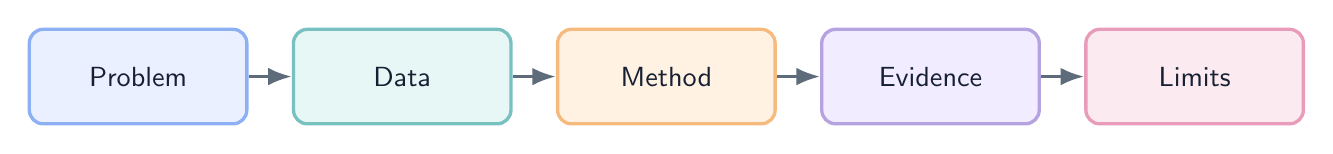
\begin{tikzpicture}[node distance=5.5mm]
\node[flowblue,text width=2.2cm] (p) {Problem};
\node[flowteal,text width=2.2cm,right=of p] (data) {Data};
\node[floworange,text width=2.2cm,right=of data] (method) {Method};
\node[flowpurple,text width=2.2cm,right=of method] (evi) {Evidence};
\node[flowpink,text width=2.2cm,right=of evi] (lim) {Limits};
\draw[arrow] (p)--(data);\draw[arrow] (data)--(method);\draw[arrow] (method)--(evi);\draw[arrow] (evi)--(lim);
\end{tikzpicture}
\end{adjustbox}
\end{center}

\begin{enumerate}
  \item 具体的な利用場面から説明する。
  \item 入力、出力、成功条件を明確にする。
  \item 構成図でデータの流れを説明する。
  \item 表や曲線でベースラインとの比較を示す。
  \item デモでは代表的な例を示し、正式な評価も別途行う。
  \item 失敗例と、次に行う価値のある実験を示す。
\end{enumerate}


% ================================================================
% APPENDICES
% ================================================================
\appendix
\titleformat{\chapter}[display]
  {\bfseries\color{Ink}\raggedright\hyphenpenalty=10000}
  {\begin{tikzpicture}[baseline=(n.base)]\node[fill=Purple,text=white,rounded corners=4pt,inner xsep=9pt,inner ysep=4pt,font=\large\bfseries] (n) {付録 \thechapter};\end{tikzpicture}}
  {8pt}{\Huge}[\vspace{3pt}\color{Line}\titlerule]

\chapter{用語集}

\begin{longtable}{>{\bfseries\RaggedRight}p{3.6cm} p{4.1cm} p{8cm}}
\toprule
英語 & 日本語 & 説明 \\
\midrule
\endfirsthead
\toprule
英語 & 日本語 & 説明 \\
\midrule
\endhead
Pixel & 画素 & 画像を構成する最小の色の単位。モデルの入力は画素の数値である。\\
Frame & フレーム & 映像を構成する1枚の静止画像。\\
FPS & フレーム毎秒 & 時間方向の細かさを決める。30 FPSは毎秒30枚を意味する。\\
BBOX & バウンディングボックス & 物体の位置を矩形で近似したもの。\\
Keypoint & キーポイント & 手首やコートの交点など、意味を定めた点。\\
Segmentation mask & 領域分割マスク & 対象に属する画素の領域を細かく示すもの。\\
Confidence & 信頼度 & モデル内部の順位付けのスコア。校正された正解確率とは限らない。\\
IoU & 共通部分と和集合の比 & 二つの矩形の共通面積を、和集合の面積で割った値。\\
NMS & 非極大値抑制 & 同じ対象の周囲にある重複候補を除く処理。\\
Homography & ホモグラフィ & 平面の座標を別の平面へ写す射影変換。\\
BEV & 鳥瞰図 & コートをほぼ真上から見た共通座標の表現。\\
Footpoint & 足元の代表点 & 選手が床に接している位置を表すための点。\\
Tracking & 追跡 & フレーム間で同じ対象のIDを維持すること。\\
Track ID & 追跡ID & 映像内の一時的な識別子。実名や背番号ではない。\\
Data association & データの対応付け & どの検出をどの追跡につなぐかを決める処理。\\
Kalman Filter & カルマンフィルタ & 動的モデルで状態を予測し、観測で補正する推定器。\\
Hungarian algorithm & ハンガリアン法 & 一対一の制約の下で合計コストが最小の対応を求める。\\
ReID & 再識別 & 外観特徴で、遮蔽後などにIDを再接続する手掛かりを得る。\\
Embedding & 埋め込みベクトル & 画像を、距離を比較できる特徴ベクトルに変換したもの。\\
Clustering & クラスタリング & 正解ラベルなしで、特徴の類似性に基づいて群に分けること。\\
Pose estimation & 姿勢推定 & 人体の関節などのキーポイント位置を予測すること。\\
Reprojection error & 再投影誤差 & 投影した位置と、既知の正解位置との差。\\
Baseline & ベースライン & 比較の基準となる、妥当で簡潔な手法。\\
Ablation & アブレーション & 構成要素を外し、改善への寄与を調べる実験。\\
Domain shift & ドメインシフト & 学習時と利用時で会場、照明、カメラ、ユニフォームなどが異なること。\\
\bottomrule
\end{longtable}

\chapter{ツール選択の早見表}

\begin{tabularx}{\textwidth}{>{\bfseries\RaggedRight}p{3cm} Y Y Y}
\toprule
目的 & 主な候補 & 利点 & 注意点 \\
\midrule
矩形データの作成 & Roboflow / CVAT & 操作画面、共同作業、形式変換が充実 & 大量作業の前に規則を定める。\\
検出器の比較研究 & MMDetection & モデルと設定が豊富 & 設定が複雑で、導入時に整理が必要。\\
YOLOの基準手法を作る & Ultralytics & 学習・推論・追跡のAPIが統一 & 更新が速いため、環境と設定を固定する。\\
幾何・カメラ処理 & OpenCV & 成熟した多言語の関数群 & 計算の成功は点の妥当性を保証しない。\\
固定カメラのリアルタイム追跡 & ByteTrack & 簡潔で追加の計算負担が小さい & 外観を使わず、長い遮蔽でIDが変わりやすい。\\
移動カメラやID交換への対処 & BoT-SORT & カメラ移動補償と任意のReID & パラメータと計算量が増える。\\
近距離・単独人物の姿勢 & MediaPipe & 軽量で統合しやすい & 試合の複数人物の高精度推定とは異なる。\\
複数人物の姿勢研究 & MMPose / OpenPose系 & モデル選択と研究の自由度が高い & 遠方、小人物、遮蔽は依然として難しい。\\
実験管理 & W\&B / MLflow & 設定、曲線、成果物を保存 & 命名規則とデータ版を先に統一する。\\
\bottomrule
\end{tabularx}

\chapter{評価指標の早見表}

\begin{tabularx}{\textwidth}{>{\bfseries\RaggedRight}p{3.3cm} Y Y}
\toprule
タスク & 推奨指標 & 併せて確認する失敗例 \\
\midrule
検出 & 適合率、再現率、AP / mAP、小物体の再現率 & 遠方のボール、重なる選手、審判を選手とする誤検出。\\
追跡 & IDF1、HOTA、IDの入れ替わり、追跡率 & 遮蔽、交差、カメラ移動。\\
ホモグラフィ & 検証点の再投影誤差、コート位置誤差 & 視野の端、外挿領域、カメラの移動。\\
チーム分類 & 正解率、macro F1、切替率、判定保留率 & 白いユニフォーム、影、審判、背面。\\
姿勢推定 & PCK、OKS、keypoint AP、角度誤差 & 遮蔽、見切れ、身体の回転。\\
イベント時刻 & フレームMAE、許容誤差内の正解率 & シュート動作の違い、一時的なボール消失。\\
システム全体 & 課題達成率、最終分析誤差、利用者の所要時間 & 前段の誤りが結論へ及ぼす影響。\\
\bottomrule
\end{tabularx}

\chapter{発展的なプロジェクトの例}

\begin{enumerate}
  \item \textbf{選手位置：}矩形の下辺中央、足首のキーポイント、領域分割による足元の点で、BEV誤差を比較する。
  \item \textbf{追跡の安定性：}固定・移動カメラで、SORT、ByteTrack、BoT-SORTのIDF1を比較する。
  \item \textbf{チーム識別：}HSV、深層特徴、追跡単位の投票を比較する。
  \item \textbf{ボール保持：}ボールと選手の距離、遮蔽、時系列状態から保持者を推定する。
  \item \textbf{シュートのイベント：}ボール軌跡、手首との距離、姿勢からリリースフレームを求める。
  \item \textbf{空間分析：}BEVの軌跡から、スペーシング、ペイントエリアの占有、トランジション速度を求める。
  \item \textbf{姿勢の安定性：}単一フレーム、移動平均、信頼度を使った時間フィルタで、関節の揺れと角度誤差を比較する。
  \item \textbf{不確実性：}位置の区間とイベントの信頼度を出し、根拠が足りない場合は判定を保留できるようにする。
\end{enumerate}

\renewcommand{\bibname}{参考文献・関連資料}
\small
\begin{thebibliography}{99}
\phantomsection\addcontentsline{toc}{chapter}{参考文献・関連資料}
\bibitem{ransac} Martin A. Fischler and Robert C. Bolles. Random Sample Consensus: A Paradigm for Model Fitting with Applications to Image Analysis and Automated Cartography. \textit{Communications of the ACM}, 1981.
\bibitem{hog} Navneet Dalal and Bill Triggs. Histograms of Oriented Gradients for Human Detection. CVPR, 2005.
\bibitem{rcnn} Ross Girshick et al. Rich Feature Hierarchies for Accurate Object Detection and Semantic Segmentation. CVPR, 2014.
\bibitem{fasterrcnn} Shaoqing Ren et al. Faster R-CNN: Towards Real-Time Object Detection with Region Proposal Networks. NeurIPS, 2015.
\bibitem{yolo} Joseph Redmon et al. You Only Look Once: Unified, Real-Time Object Detection. CVPR, 2016.
\bibitem{detr} Nicolas Carion et al. End-to-End Object Detection with Transformers. ECCV, 2020.
\bibitem{sort} Alex Bewley et al. Simple Online and Realtime Tracking. ICIP, 2016.
\bibitem{deepsort} Nicolai Wojke, Alex Bewley, and Dietrich Paulus. Simple Online and Realtime Tracking with a Deep Association Metric. ICIP, 2017.
\bibitem{bytetrack} Yifu Zhang et al. ByteTrack: Multi-Object Tracking by Associating Every Detection Box. ECCV, 2022.
\bibitem{botsort} Nir Aharon, Roy Orfaig, and Ben-Zion Bobrovsky. BoT-SORT: Robust Associations Multi-Pedestrian Tracking. arXiv:2206.14651, 2022.
\bibitem{hota} Jonathon Luiten et al. HOTA: A Higher Order Metric for Evaluating Multi-Object Tracking. International Journal of Computer Vision, 2021.
\bibitem{openpose} Zhe Cao et al. OpenPose: Realtime Multi-Person 2D Pose Estimation Using Part Affinity Fields. IEEE TPAMI, 2021.
\bibitem{hrnet} Ke Sun et al. Deep High-Resolution Representation Learning for Human Pose Estimation. CVPR, 2019.
\bibitem{blazepose} Valentin Bazarevsky et al. BlazePose: On-device Real-time Body Pose Tracking. arXiv:2006.10204, 2020.
\bibitem{integralpose} Xiao Sun et al. Integral Human Pose Regression. ECCV, 2018.
\bibitem{simcc} Yanjie Li et al. SimCC: a Simple Coordinate Classification Perspective for Human Pose Estimation. ECCV, 2022.
\bibitem{vitpose} Yufei Xu et al. ViTPose: Simple Vision Transformer Baselines for Human Pose Estimation. NeurIPS, 2022.
\bibitem{rtmpose} Tao Jiang et al. RTMPose: Real-Time Multi-Person Pose Estimation Based on MMPose. arXiv:2303.07399, 2023.
\bibitem{opencv} OpenCV Documentation. Basic Concepts of the Homography Explained with Code. \url{https://docs.opencv.org/4.x/d9/dab/tutorial_homography.html}
\bibitem{ultralytics} Ultralytics Documentation. Multi-Object Tracking with BoT-SORT and ByteTrack. \url{https://docs.ultralytics.com/modes/track/}
\bibitem{roboflow} Roboflow Documentation. Annotation Tools and Project Types. \url{https://docs.roboflow.com/annotate/annotation-tools}
\end{thebibliography}
\normalsize

\begin{heroBox}
\textbf{おわりに：}\quad
本教材は、継続して発展させられる分析の枠組みを示した。まず課題と出力を定義し、それに合うデータと手法を選ぶ。中間結果を残して段階ごとに評価し、根拠に基づいて結論を述べ、システムの限界も明確にする。
\end{heroBox}

\end{document}
